\documentclass[11pt,a4paper]{article}

% ════════════════════════════════════════════════════════════════════
%  Federated Solar-Flare Prediction on SWAN-SF: A Provenance,
%  Leakage, and Evaluation-Protocol Audit (v3.9)
%  arXiv-preprint-style single-column manuscript
% ════════════════════════════════════════════════════════════════════

\usepackage{graphicx}
\usepackage{xcolor}
\usepackage{geometry}
\usepackage{amsmath}
\usepackage{amssymb}

\geometry{a4paper, top=2.6cm, bottom=2.6cm, left=2.5cm, right=2.5cm}
% left and right margins are symmetric (iron rule)

\usepackage{booktabs}
\usepackage{tabularx}
\usepackage{longtable}
\usepackage{adjustbox}
\usepackage{enumitem}
\usepackage{caption}
\usepackage{microtype}
\usepackage{xurl}          % allow URLs to break at any character
\usepackage{placeins}   % \FloatBarrier at each section
\usepackage{needspace}

\captionsetup{font=small, labelfont=bf, skip=6pt}

% Bibliography: numeric citations, arXiv preprint style
\usepackage[numbers,sort&compress]{natbib}
\bibliographystyle{unsrtnat}

% hyperref ALWAYS last among content packages
\usepackage[
    colorlinks=true,
    linkcolor=blue!55!black,
    citecolor=blue!45!black,
    urlcolor=blue!55!black,
    bookmarks=true,
    bookmarksnumbered=true,
    unicode=true,
    pdftitle={Federated Solar-Flare Prediction on SWAN-SF: A
              Provenance, Leakage, and Evaluation-Protocol Audit},
    pdfauthor={Deepanshu Balhara, Davesh Vats},
    pdfsubject={Federated Learning, Solar Flare Prediction, Smart Grid
                Protection, Space Weather},
    pdfkeywords={federated learning, solar flare prediction, smart grid,
                 GIC, FedProx, SWAN-SF, data locality}
]{hyperref}

% Orphan/widow prevention
\widowpenalty=10000
\clubpenalty=10000

% Allow emergency line stretching to avoid overfull boxes
\emergencystretch=1.8em

% Ragged-bottom: avoid stretched vertical glue
\raggedbottom

% Slight paragraph spacing for preprint readability
\setlength{\parindent}{1.2em}
\setlength{\parskip}{2pt plus 1pt}

% ── Custom math macros ──────────────────────────────────────────────
\newcommand{\R}{\mathbb{R}}
\newcommand{\E}{\mathbb{E}}
\newcommand{\w}{\mathbf{w}}
\newcommand{\norm}[1]{\left\lVert #1 \right\rVert}
\newcommand{\Fbeta}{F_{\beta}}

\title{Federated Solar-Flare Prediction on SWAN-SF: A Provenance,
Leakage, and Evaluation-Protocol Audit}
\author{Deepanshu Balhara \and Davesh Vats}
\date{October 2026}

\begin{document}

% ════════════════════════════════════════════════════════════════════
%  CUSTOM TITLE BLOCK (arXiv-preprint aesthetic, page 1)
% ════════════════════════════════════════════════════════════════════
\thispagestyle{plain}

\begin{center}
    {\color{black!85}\rule{\textwidth}{0.4pt}}\\[2.2em]
    {\LARGE\bfseries Federated Solar-Flare Prediction on SWAN-SF:\\[0.35em]
     A Provenance, Leakage, and Evaluation-Protocol Audit\par}
    \vspace{1.6em}
    {\large Deepanshu Balhara\textsuperscript{1} \quad and \quad
     Davesh Vats\textsuperscript{2}\par}
    \vspace{0.7em}
    {\small\textit{Independent Researchers}\textsuperscript{1,2}\par}
    % NOTE FOR AUTHORS: replace the affiliation line above with your
    % institutional affiliations and contact e-mails before posting.
    \vspace{1.1em}
    {\small October 2026\par}
    \vspace{1.4em}
    {\color{black!85}\rule{\textwidth}{0.4pt}}
\end{center}

\vspace{0.4em}

\begin{center}
\begin{minipage}{0.92\textwidth}
\footnotesize
\textbf{Abstract ---}
Grid-resilience operators need flare-probability components trained on
magnetogram histories, and data-locality constraints can preclude
pooling the underlying observations. We audit what actually happens
when federated learning meets the public SWAN-SF benchmark. Six
\emph{simulated} regional clients hold disjoint Dirichlet-skewed shards
of the cleaned benchmark under a frozen protocol: immutable splits,
validation-only selection and calibration, a runtime leakage audit, and
single-pass test evaluation. A provenance audit against the raw
benchmark (normalisation-invariant instance matching, 98.7--100\%
coverage, 100\% label agreement) shows the cleaned export's
same-partition train/test pairing shares instances: every flaring test
window (6{,}234) also appears in training, and 85.7--90\% of training
positives are TimeGAN-synthetic. On a leakage-free fold (training
partitions 1--4, single-pass test on partition 5) discrimination
generalises for all arms (ROC-AUC 0.906--0.978) and the
federated-versus-centralised gap disappears. A BatchNorm-transport
diagnostic then shows the in-partition FedAvg collapse (test ROC-AUC
0.575) to be an evaluation artefact: the same weights score 0.951 under
correct normalisation, FedAvg's weights never lose discriminative
content (0.953 at round 50), and a controlled no-BatchNorm run leaves
both FedAvg and FedProx stable and near-identical --- the published
algorithm gap is substantially mediated by untransported BN statistics,
a saturated validation monitor, and the checkpoint rule that monitor
feeds. On the raw, unbalanced substrate the outcome is
encoder-conditional: federated MLP arms degrade while LSTM arms recover
(FedProx-LSTM 0.970/0.404). Calibration, not detection, is the
deployability boundary. Prior federated flare forecasting exists (Fu et
al., 2023 preprint); this is the first federated evaluation on SWAN-SF
and the first with a provenance audit. An independent byte-verified
re-execution reproduces every headline metric.

\vspace{0.55em}
\noindent\textbf{Keywords:} federated learning; solar flare prediction;
SWAN-SF; data provenance; evaluation audit; BatchNorm; non-IID data;
class imbalance; data locality

\vspace{0.55em}
\noindent\footnotesize Source code and all experimental artefacts:
\url{https://github.com/Daveshvats/Federated-Learning-for-Distributed-Space-Weather-Monitoring}
\end{minipage}
\end{center}

\vspace{0.8em}

% ════════════════════════════════════════════════════════════════════
% SECTION 1 — INTRODUCTION
% ════════════════════════════════════════════════════════════════════
\section{Introduction}\label{sec:intro}

Modern society has quietly built its electrical backbone in the path of
a cosmic hazard. Geomagnetically induced currents (GICs) are
quasi-direct currents that flow in high-voltage transmission lines when
a geomagnetic storm---itself driven by the arrival of a coronal mass
ejection (CME) associated with a major solar flare---distorts the
Earth's magnetosphere. The time-varying geomagnetic field induces
geo-electric fields in the conducting crust, and these fields drive GICs
through grounded transformer neutrals. Once inside a high-voltage
transformer, even a modest GIC biases the alternating flux into
half-cycle saturation, producing harmonics, reactive-power absorption,
and localized heating that can culminate in irreversible thermal
damage~\cite{bolduc2002,boteler2019}. The canonical demonstration of
this failure mode remains the 13~March 1989 storm, which collapsed the
Hydro-Qu\'ebec grid in ninety seconds and left six million customers
without power for nine hours~\cite{bolduc2002,boteler2019}. The
July~2012 event, an eruptive flare/CME of Carrington-class magnitude
that missed Earth's orbital position by roughly nine days, is a stark
reminder that the next exposure is a matter of when, not
if~\cite{baker2013}.

The first line of defence against such events is forecasting. Grid
operators who receive an early warning that an M- or X-class flare has
erupted, or is likely to erupt, in a magnetically complex active region
can pre-emptively derate transformers, adjust reserve margins, postpone
switching operations, and prepare load-shedding plans in the
window between the flare observation and the CME's arrival one to three
days later. Machine-learning flare-prediction models built on
photospheric vector-magnetogram summaries---the SHARP parameter
suite~\cite{bobra2015} and its descendants---have demonstrated
statistically skilful classification of flaring versus non-flaring
active regions~\cite{leka2019,georgoulis2021}. The predictive signal
lives in quantities such as total unsigned current helicity, magnetic
free energy, and flux-emergence proxies, all of which are computed
routinely by solar observatories on every continent and in orbit.

There is, however, a structural obstacle to training the strongest
possible model: many institutions that could pool their data choose
not to. The highest-fidelity flare-forecasting observations are
produced and curated by nationally mandated agencies---NASA and NOAA
in the Americas, ESA in Europe, JAXA in the Asia-Pacific region, ISRO
in South Asia, KASI in East Asia, and the Australian Bureau of
Meteorology (BoM) in Oceania---and in several jurisdictions the raw
magnetogram-derived time series are treated as nationally sensitive
assets whose redistribution is restricted by data-locality policies,
inter-agency agreements, or export controls. Whether these
restrictions are legally binding or a matter of institutional policy,
the practical effect is the same: if the custodians do not pool, each
either trains on its own regional shard or forgoes machine learning
altogether, and the community inherits models that each see a biased
slice of the active-region population. The present study does not
claim that any specific agency's flare data cannot be pooled; it takes
data locality as a plausible deployment constraint and studies its
consequences under a controlled simulation of that constraint.

Federated learning (FL)~\cite{mcmahan2017,kairouz2021} is precisely the
mechanism for this setting. In cross-silo FL, each data-holder trains a
shared model architecture locally and transmits only parameter updates
to an aggregation server, which averages them into a new global model.
Raw measurements never leave the custodian's infrastructure. FL has
already proven transformative in medicine and digital health, where
patient-privacy constraints are structurally similar to the
data-locality constraints just described~\cite{rieke2020}. What has
not existed, prior to the present work and per the documented search
protocol of Section~\ref{sec:related}, is a systematic treatment of FL
for solar flare prediction---the solar-physics community's benchmark
workflows \cite{leka2019,georgoulis2021,angryk2020} are all centrally
pooled, and we found no application of FL to photospheric flare
forecasting in the FL literature.

This paper closes that gap. We present a complete, reproducible
federated framework---implemented, versioned, and released as open
source---that \emph{simulates} six regional data custodians (labelled
A--F by region; no real institution participates), each holding a
non-IID shard of the SWAN-SF benchmark \cite{angryk2020} in its cleaned
and rebalanced form, and evaluates whether federation can approach the
centralised upper bound without any data movement. The framework is an
upstream flare-probability component: it emits calibrated M/X flare
probabilities and fixed-false-positive-rate alerting points that a
future geomagnetic-hazard pipeline (CME/interplanetary propagation,
storm forecasting, GIC and power-system response modelling) could
consume; the downstream chain is not evaluated here. The specific
contributions are:

\begin{enumerate}[leftmargin=2em, itemsep=3pt]
  \item \textbf{A problem formulation and system architecture} that maps
  grid-resilience precursor alerting onto a cross-silo federated
  classification problem with a safety-critical, recall-weighted
  objective, and that operationalises the data-locality constraint as a
  concrete, simulable protocol (Section~\ref{sec:problem} and
  Section~\ref{sec:method}).
  \item \textbf{A non-IID federation protocol for SWAN-SF} that combines
  Dirichlet label-skew partitioning across six simulated regional
  clients, a server-aware Fed-Focal loss \cite{sarkar2020} for extreme
  class imbalance, and optional distribution-aware aggregation and
  per-client SMOTE oversampling (both studied as ablation arms; the
  SMOTE arm is inert on this benchmark variant), on top of both FedAvg
  \cite{mcmahan2017} and FedProx \cite{li2020} training loops
  (Section~\ref{sec:method}).
  \item \textbf{A frozen, leakage-audited evaluation protocol}: an
  immutable train/validation/test contract, calibration and threshold
  selection on validation only, single-pass test evaluation, a
  centralised-MLP architecture control, five-seed statistics with
  confidence intervals and paired significance tests, a 24-cell
  component-ablation grid, and---as protocol extensions released with
  this revision---region-disjoint splits, natural-prevalence validation
  with frozen FPR operating points, untouched client holdouts, an
  explicit training-budget audit, event-level alerting metrics, and a
  calibration-comparison harness (Section~\ref{sec:experiments}).
  \item \textbf{A data-locality cost study.} On the held-out test
  partitions (331{,}185 windows, 1.88\% prevalence), FedProx attains a
  ROC-AUC of 0.954---97.7\% of the centralised XGBoost reference
  (0.977)---and did not underperform the pooled centralised MLP of
  identical architecture (0.888) on this benchmark and configuration,
  a comparison whose optimisation budgets are documented and not
  matched, while plain FedAvg diverges during training (validation AUC
  $0.99\to0.05$); FedProx exceeds FedAvg's PR-AUC on all five seeds
  (one-sided Wilcoxon $p=0.031$)
  (Section~\ref{sec:results}).
  \item \textbf{A cross-model interpretability audit.} SHAP analysis
  of both the centralised XGBoost reference and the federated global
  model, with physical-parameter-group aggregation, shows both
  concentrate decisions on current helicity, the Schrijver
  flux-emergence proxy \cite{schrijver2007}, and Lorentz-force
  components---consistent with established flare physics
  (Section~\ref{sec:results}).
\end{enumerate}

We are explicit about what is \emph{not} claimed: per-client SMOTE
contributes nothing on this benchmark variant (zero synthetic samples;
reported as a null result, not a contribution); the verified property
is data locality, not cryptographic privacy; the six clients are
simulated, not real agencies; and the downstream
flare$\to$CME$\to$storm$\to$GIC chain is discussed as future
integration, not evaluated.

In addition to these scientific contributions, the released framework
embodies a documented engineering narrative: a multi-version stability
iteration (v2.1--v3.1) in which Dirichlet concentration, focal-loss
alpha clamping, optimiser choice for variance-reduced FL, and dataset
auditing were each adjusted in response to diagnosed failure modes. We
summarise this evolution in Appendix~\ref{sec:appendix} because it
constitutes, in our view, transferable know-how for practitioners
attempting the first FL deployment in any physical-science domain.

The remainder of the paper is organised as follows.
Section~\ref{sec:related} reviews flare prediction and federated
learning. Section~\ref{sec:problem} formalises the problem.
Section~\ref{sec:method} details the system architecture and
methodology. Section~\ref{sec:experiments} describes the experimental
setup, Section~\ref{sec:results} presents and analyses results, and
Section~\ref{sec:discussion} discusses operational integration and
engineering lessons. Section~\ref{sec:limitations} states limitations
and future work, and Section~\ref{sec:conclusion} concludes.

% ════════════════════════════════════════════════════════════════════
% SECTION 2 — BACKGROUND AND RELATED WORK
% ════════════════════════════════════════════════════════════════════
\section{Background and Related Work}\label{sec:related}

\subsection{Solar flare prediction from photospheric magnetograms}

The physical premise of data-driven flare forecasting is that the
photospheric magnetic field of an active region encodes the stress
budget that a future flare will release. Schrijver~\cite{schrijver2007}
demonstrated that a single scalar---the R-value, the unsigned flux
within high-gradient polarity-separation corridors---separates
major-flaring regions from non-flaring ones with striking reliability,
and this proxy remains among the strongest single flare predictors
identified to date. Bobra and Couvidat~\cite{bobra2015} operationalised
the machine-learning view of the problem, showing that a support-vector
machine trained on 25~SHARP parameters derived from SDO/HMI vector
magnetograms can forecast M-class flares with useful skill, and that
feature selection matters as much as model choice. Subsequent
community-wide blind tests, most notably the multi-method comparison of
Leka et al.~\cite{leka2019}, established two durable findings: (i)~no
single method dominates across all event definitions and skill
metrics, and (ii)~the effective ceiling on skill is set by the quality
and homogeneity of the training data rather than by classifier
complexity.

The European FLARECAST project~\cite{georgoulis2021} pushed the
operational agenda further, combining multiple forecasting methods and
data sources in an open framework, and it explicitly confronted the
data-heterogeneity problem that motivates the present paper. On the
data side, the SWAN-SF benchmark of Angryk et
al.~\cite{angryk2020} released a multivariate time-series dataset of
roughly 8{,}000 active-region tracks with 24 physical parameters per
timestep and flare-history labels, specifically designed to make flare
prediction reproducible and comparable; it has since become the
community's reference benchmark, and a family of cleaned and rebalanced
variants (random undersampling, Tomek-link cleaning, and TimeGAN-based
synthetic augmentation \cite{yoon2019}) has been curated to make the
benchmark tractable for supervised learning. Recent deep-learning work
on SWAN-SF continues to raise the centralised ceiling: contrastive
pretraining and multifaceted preprocessing \cite{eskandari2024} and
LSTM-style temporal architectures \cite{hassani2025} exploit the
sequential structure of the 60-minute observation windows. All of these
works, without exception, assume that the full training corpus is
available in one place.

\subsection{Federated learning under statistical heterogeneity}

Federated learning was introduced by McMahan et
al.~\cite{mcmahan2017} in the FedAvg formulation: clients perform
several epochs of local SGD on private data, and a server aggregates
the resulting weights by sample-size-weighted averaging. The defining
difficulty, identified almost immediately, is statistical
heterogeneity: when client data distributions differ---the non-IID
setting---local optima diverge from the global optimum, and naive
averaging can oscillate or diverge \cite{zhao2018}. FedProx
\cite{li2020} addresses this by adding a proximal term
$(\mu/2)\norm{\w-\w^{(t)}}^{2}$ to each client's local objective that
anchors local training to the current global model, tolerating partial
work and heterogeneous local computation. SCAFFOLD \cite{karimireddy2020}
attacks the same problem with control variates that correct client
drift using variance reduction. The comprehensive survey of Kairouz et
al.~\cite{kairouz2021} situates these algorithms within the broader
open-problem landscape, including robust aggregation, personalisation,
and privacy. Cross-silo FL---few, reliable, institutionally owned
clients---is the deployment regime relevant to space-weather agencies,
and it contrasts with the cross-device regime in its stability
requirements and long-lived participants.

\subsection{Class imbalance in federated learning}

Flare prediction inherits an extreme class-imbalance regime: in
SWAN-SF's natural test distribution, roughly 1.9\% of windows precede
M/X-class flares, while the rebalanced training partitions sit near
parity. The focal loss of Lin et al.~\cite{lin2017}, originally
developed for dense object detection, down-weights easy examples with a
$(1-p_t)^{\gamma}$ modulating factor and concentrates gradient on hard
positives; it has become the default imbalance workhorse. Sarkar et
al.~\cite{sarkar2020} adapted focal loss specifically to FL in the
Fed-Focal formulation, in which the class-weighting parameter is
adjusted using information available at the server about the global
class distribution, so that clients with different local positivity
rates do not implicitly reweight the global objective. In parallel,
synthetic oversampling remains a standard pre-processing response:
SMOTE \cite{chawla2002} interpolates minority-class neighbours, and
mixup \cite{zhang2018} creates convex combinations of training pairs.
Under federation, rebalancing must be applied locally per client, since
the pooled distribution is precisely what no participant can inspect.

\subsection{Positioning of this work and search protocol}
\label{sec:litsearch}

Two research threads---physics-grounded flare prediction and
heterogeneity-robust federated learning---have developed largely
independently, and we are not aware of any prior work that joins them.
Because the first-FL-treatment claim is a factual statement about the
literature, we document the search protocol behind it rather than
relying on ``to the best of our knowledge''. The search was last
repeated on 29~September 2026 across general web, arXiv, NASA ADS,
and publisher indexes (ScienceDirect, IEEE) reached through a web
search engine, using four query strings: (i)~\emph{federated learning
solar flare prediction}; (ii)~\emph{federated learning space weather
forecasting}; (iii)~\emph{federated learning SWAN-SF benchmark
magnetogram}; (iv)~\emph{cross-silo federated learning geophysics
heliophysics distributed observatories}. Records were included if
they apply federated or distributed multi-client learning without raw
data pooling to flare prediction or space-weather forecasting; records
were excluded if they concern centralised machine learning for flares
(the case for all entries of query~i), federated forecasting of
\emph{solar power or irradiance}, federated \emph{terrestrial}
weather forecasting, or federated computing on spacecraft without a
scientific forecasting task (the categories returned by query~ii).
Screening the 30 records returned by the four queries yielded
\emph{zero} in-scope records; the raw result listings are committed
with the repository (\texttt{docs/lit\_search/}). We note two
limitations of this protocol: web-engine coverage of grey literature
is incomplete, and the screening was single-reviewer, so a
PRISMA-style dual-screened log remains queued repository work. Within
those limits, the present work is the first federated treatment of
solar flare prediction, the first FL framework evaluated on the
SWAN-SF benchmark, and the first to quantify the cost of the
data-locality constraint---the gap between federated and centralised
skill---specifically for a safety-critical smart-grid application. In
doing so it also contributes a rarely documented artifact: an honest
engineering log of the failure modes encountered when FL meets a
severely imbalanced physical-science benchmark (Appendix~\ref{sec:appendix}).

% ════════════════════════════════════════════════════════════════════
% SECTION 3 — PROBLEM FORMULATION
% ════════════════════════════════════════════════════════════════════
\section{Problem Formulation}\label{sec:problem}

\subsection{Federated risk minimisation}

Let $K$ denote the number of participating clients (simulated shards
of the pooled benchmark), each
holding a private dataset
$\mathcal{D}_k = \{(x_i, y_i)\}_{i=1}^{n_k}$ of active-region
observation windows $x_i \in \R^{d}$ and binary labels
$y_i \in \{0,1\}$ indicating whether an M- or X-class flare occurs
within the forecasting horizon. Let
$\mathcal{D} = \bigcup_{k=1}^{K} \mathcal{D}_k$ with
$n = \sum_k n_k$. The goal of standard centralised learning is to
solve
\begin{equation}\label{eq:central}
    \min_{\w \in \R^{p}} \;
    F(\w) \;=\; \frac{1}{n}\sum_{i=1}^{n}
    \ell\big(f_{\w}(x_i),\, y_i\big),
\end{equation}
where $f_{\w}$ is the prediction model, $\ell$ a per-sample loss, and
$p$ the number of parameters. In the federated setting this objective
is decomposed as a weighted sum of local empirical risks
\begin{equation}\label{eq:fedobj}
    \min_{\w} \; F(\w) \;=\; \sum_{k=1}^{K} \rho_k \, F_k(\w),
    \qquad
    F_k(\w) \;=\; \frac{1}{n_k}\sum_{(x_i,y_i)\in\mathcal{D}_k}
    \ell\big(f_{\w}(x_i),\, y_i\big),
\end{equation}
with aggregation weights $\rho_k \ge 0$, $\sum_k \rho_k = 1$. The
vanilla FedAvg choice is $\rho_k = n_k / n$; Section~\ref{sec:method}
describes the distribution-aware weights used in this work.

\subsection{The data-locality constraint}

The operational constraint that distinguishes cross-silo FL from
distributed optimisation is not an algorithmic preference but an
institutional invariant: for every round $t$ and client $k$, the
server may observe only the weight increment
$\Delta \w_k^{(t)} = \w_k^{(t+1)} - \w^{(t)}$ (or equivalently the
locally trained weights), never $x_i$ or $y_i$ for any sample in
$\mathcal{D}_k$. Formally, the communication transcript
\begin{equation}\label{eq:privacy}
    \mathcal{T} \;=\;
    \big\{\Delta \w_k^{(t)}\big\}_{k=1,\dots,K;\; t=1,\dots,T}
\end{equation}
is the only quantity that crosses the client boundary. This is the
data-locality constraint that motivates cross-silo federated learning
in settings where shards genuinely cannot be pooled---proprietary
archives, cross-border data governance, organisational silos. We
stress that no such constraint binds this benchmark: the SWAN-SF
data is public and freely poolable, and the federated protocol here
is a controlled simulation of the constraint, not a response to it.
The released framework nonetheless enforces the property by
construction: the client-side pipeline never serialises raw shards.
We further stress the scope of the property: it is
\emph{data locality}, not cryptographic privacy. The transcript
$\mathcal{T}$ itself can leak information about training data
(Section~\ref{sec:threatmodel}); defending against an adversary who
observes it requires secure aggregation or differential privacy, which
are implemented but not evaluated for accuracy cost here.

\subsection{Statistical heterogeneity}

In genuine cross-silo deployments, participating organisations sample
different populations under different label distributions, so the
local class priors $p_k = \Pr(y=1 \mid k)$ differ from the pooled
prior $\bar{p}$ --- statistical heterogeneity, the defining
difficulty of federated optimisation. Because SWAN-SF is a
single-instrument, whole-disk benchmark, no physical mechanism
produces such skew here; we therefore \emph{impose} it by
partitioning the pooled training data among $K$ clients with a
symmetric Dirichlet distribution of concentration $\alpha$
(Section~\ref{sec:method}),
so that the realised local priors span a wide range around $\bar{p}$.
The partition is a simulation instrument --- a test of federation
under heterogeneity, not a claim about how the data is produced: the
labels and windows come from one observatory pipeline for every
shard. The consequence for optimisation is well documented
\cite{zhao2018,li2020}: local objectives $F_k$ become misaligned, and
plain averaging of locally optimised weights introduces drift that
grows with the number of local epochs. FedProx counteracts this drift
by locally solving
\begin{equation}\label{eq:fedprox}
    \min_{\w} \;
    F_k(\w) \;+\; \frac{\mu}{2}\,\norm{\w - \w^{(t)}}^{2},
\end{equation}
which keeps client updates in a trust region around the global model.
The strength of this anchor, $\mu$, is a central hyperparameter of
this study.

\subsection{A safety-critical, recall-weighted objective}

Rare-event forecasting inverts the usual classification cost
structure: at 1--2\% positive prevalence an all-clear forecast is
98--99\% accurate and useless, while a missed positive is the event
the forecast exists to catch. Following rare-event evaluation
practice, we therefore evaluate with the $F_\beta$ measure
\begin{equation}\label{eq:fbeta}
    \Fbeta \;=\;
    \frac{(1+\beta^{2})\, P\, R}{\beta^{2} P + R},
    \qquad \beta = 2,
\end{equation}
where $P$ and $R$ are precision and recall; $\beta = 2$ weights recall
twice as heavily as precision. Because the deployed decision rule is a
threshold $\tau$ on the predicted flare probability, the framework
treats $\tau$ as a free, per-model parameter selected on held-out
validation evidence to maximise Eq.~\eqref{eq:fbeta}, rather than
fixing $\tau = 0.5$ by convention. Section~\ref{sec:results} shows this
choice is not cosmetic: at the conventional threshold, every federated
model trained on rebalanced local data is operationally unusable, and
threshold optimisation is what converts a well-ranked model into a
usable detector.

% ════════════════════════════════════════════════════════════════════
% SECTION 4 — SYSTEM ARCHITECTURE AND METHODOLOGY
% ════════════════════════════════════════════════════════════════════
\section{System Architecture and Methodology}\label{sec:method}

\subsection{Architecture overview}

\begin{sloppypar}
Figure~\ref{fig:arch} shows the complete system. Six regional
observatory clients---stand-ins for NASA/NOAA, ESA (PROBA-2), JAXA,
ISRO, KASI, and BoM---each hold a private, non-IID shard of the
benchmark. In every communication round, each selected client trains a
local copy of the shared model on its shard (with local rebalancing and
an imbalance-robust loss, described below), and returns only its weight
increment to the aggregation server. The server forms the next global
model with distribution-aware weighted averaging, broadcasts it to all
clients, and the cycle repeats for $T = 50$ rounds. Downstream of
federation, the global model is calibrated for operations: its flare
probabilities pass through the $F_\beta$-optimal threshold and become
GIC early-warning decisions, which plug into existing SCADA workflows
for grid management. The division of labour is
deliberate: everything that touches raw magnetogram data (loading,
rebalancing, local training) executes inside the client boundary;
everything the server touches is a weight tensor.
\end{sloppypar}

\begin{figure}[t]
    \centering
    \begin{adjustbox}{max width=\textwidth, max height=0.46\textheight}
        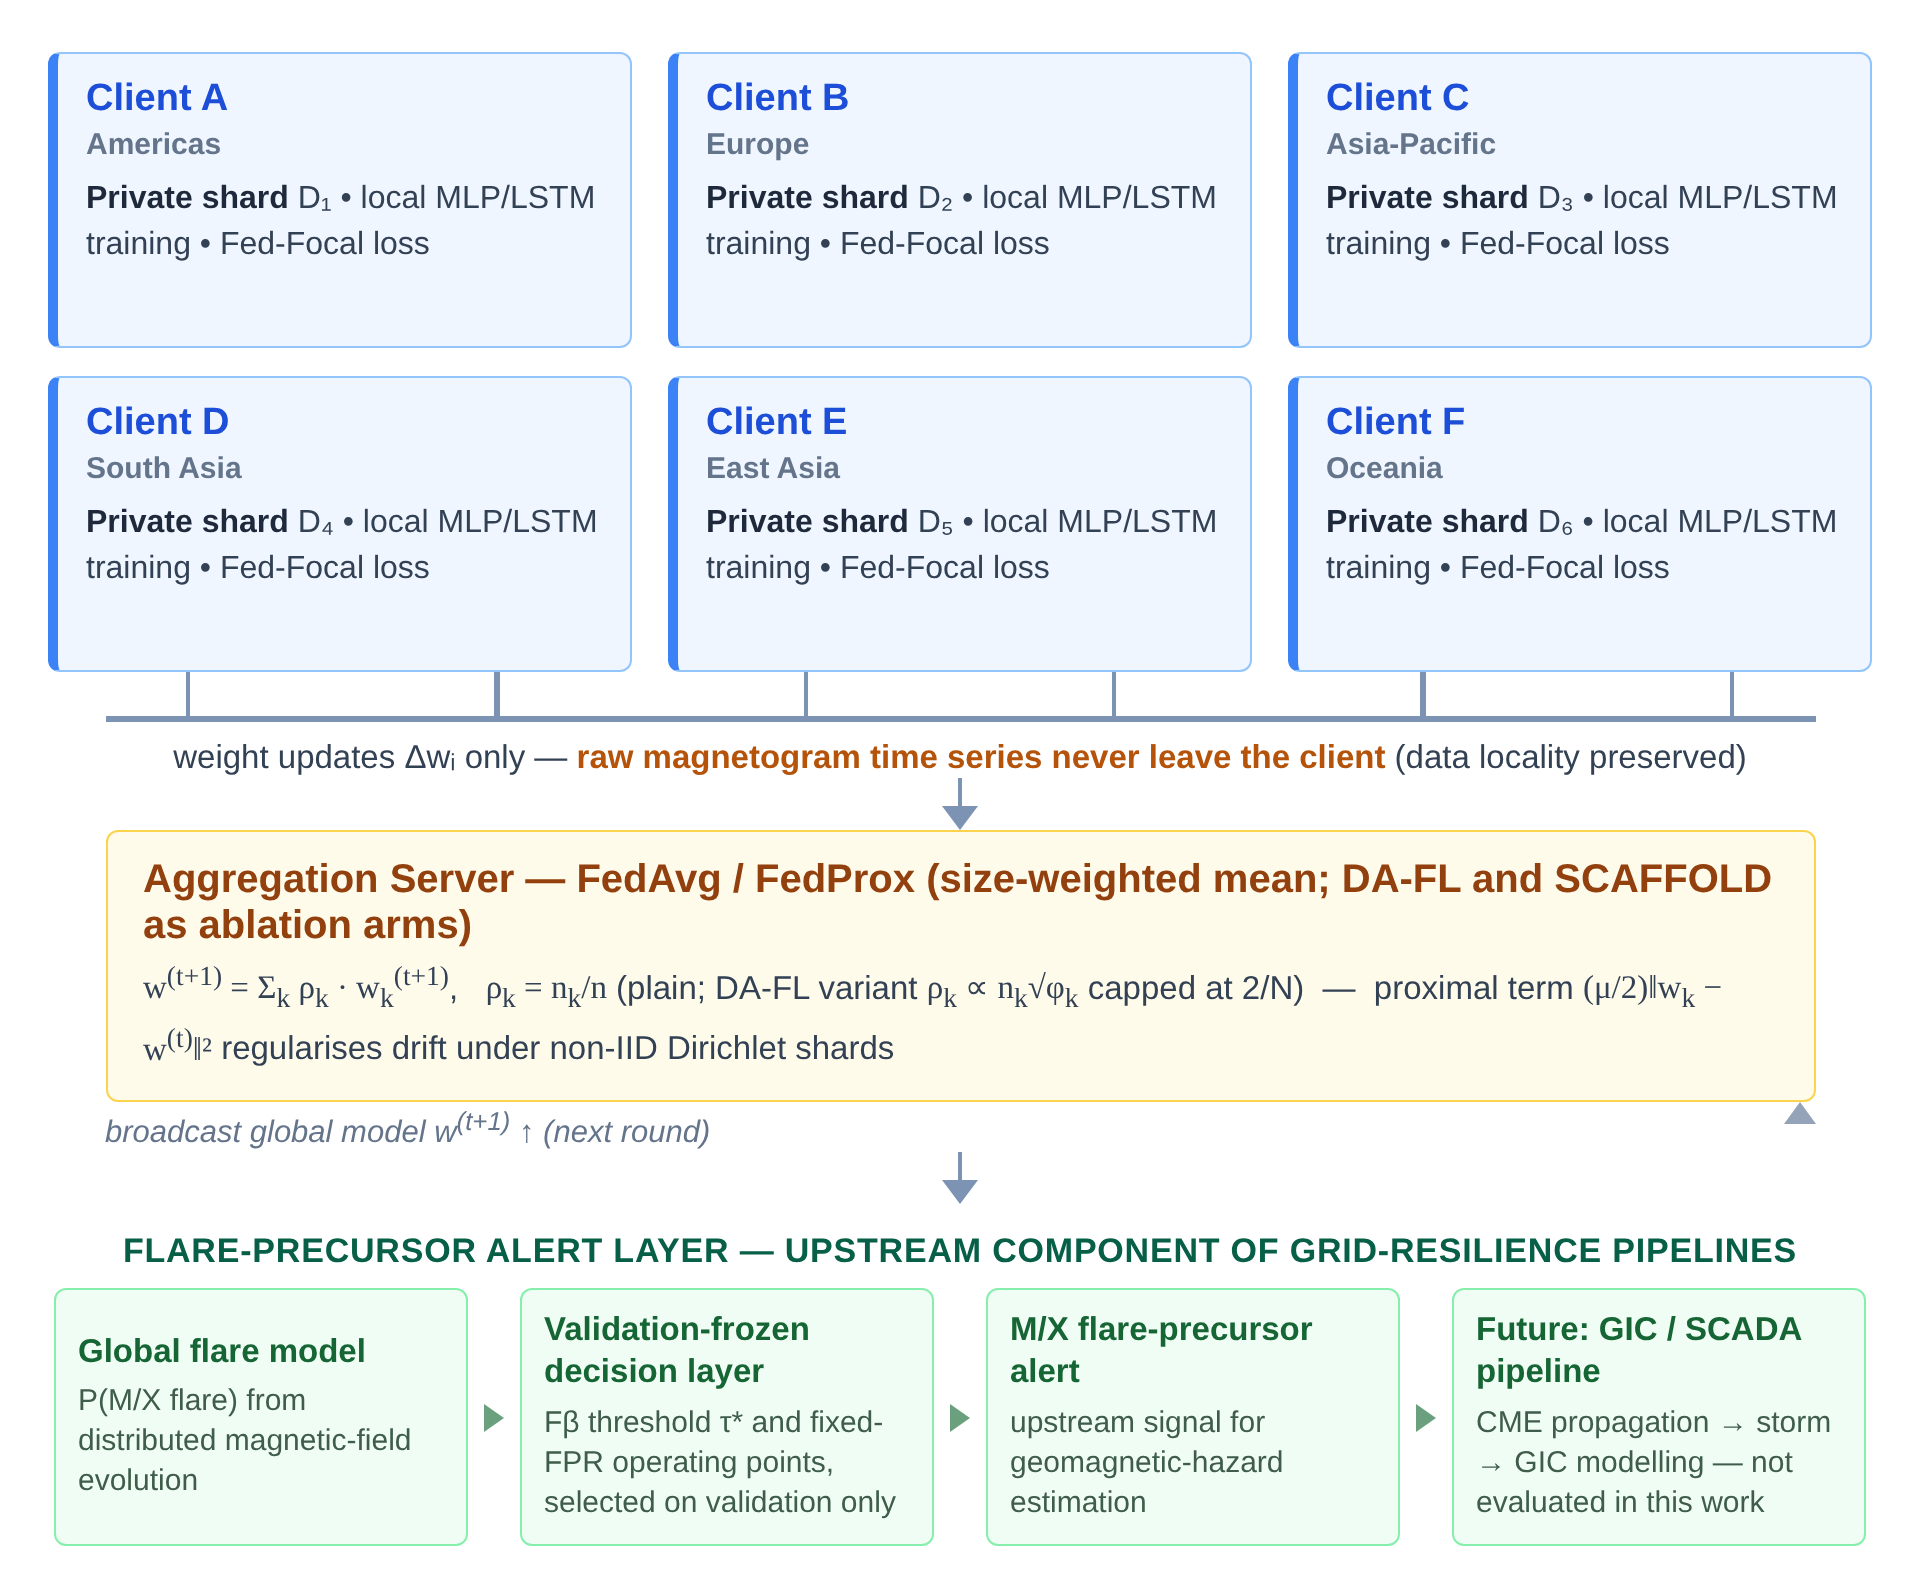
\includegraphics{figures/fig_architecture.png}
    \end{adjustbox}
    \caption{Federated space-weather monitoring architecture for
    smart-grid protection. Six regional observatory clients hold
    private non-IID shards of the benchmark; only weight updates
    $\Delta \w_k$ cross the agency boundary. The aggregation server
    applies FedAvg/FedProx with distribution-aware weighting
    ($\rho_k \propto n_k\sqrt{\phi_k}$, capped at $2/K$). The global
    model feeds an $F_\beta$-optimal decision layer for GIC early
    warning and SCADA integration.}
    \label{fig:arch}
\end{figure}

\subsection{Data: the SWAN-SF benchmark and its cleaned variant}

All experiments use the SWAN-SF benchmark \cite{angryk2020}
(doi:10.7910/DVN/EBCFKM), a multivariate time-series dataset of
active-region observation windows drawn from SDO/HMI vector
magnetograms, with 24 physically motivated parameters per timestep
sampled over 60-minute sliding windows and labels indicating the
occurrence of $\geq$M-class flares within the prediction horizon. The
24 parameters summarise magnetic-field complexity and include, among
others: total unsigned current helicity (TOTUSJH), total photospheric
magnetic free energy (TOTPOT), total unsigned vertical current
(TOTUSJZ), total unsigned flux (USFLUX), the sum of absolute
net-current-per-polarity (SAVNCPP), absolute net current helicity
(ABSNJZH), mean shear angle and the fraction of high-shear area
(MEANSHR, SHRGT45), the Schrijver flux-emergence proxy (R-value), and
the three components of the total Lorentz force (TOTFX, TOTFY, TOTFZ)
\cite{schrijver2007,bobra2015}.

We ingest the benchmark through its community-maintained cleaned
variant\footnote{Cleaned SWAN-SF Dataset,
\url{https://github.com/samresume/Cleaned-SWANSF-Dataset}, which
applies per-partition preprocessing: random undersampling with Tomek
links and TimeGAN-based synthetic augmentation for the training
partitions \cite{yoon2019}, LSBZM normalisation, and FPC-KNN
imputation.}, combining all five data partitions. The training
partitions are class-balanced by this preprocessing (pooled positive
rate $\bar{p} \approx 0.489$), while the untouched test partitions
retain the natural, severely imbalanced prevalence of approximately
$1.9\%$ flare windows across roughly $3.3\times10^{5}$ held-out
samples. This train--test contrast is not an artefact we introduce; it
is inherited from the benchmark's design philosophy, and it has a
consequence that shapes the entire evaluation: models trained at
$\sim$49\% prior must detect events at a $\sim$2\% prior, so absolute
probability calibration degrades and decision thresholds must be
re-optimised post hoc (Section~\ref{sec:thresholding}).

\subsection{Client-side feature representation}

The framework supports two representations of the same 60-timestep
observation windows. In the MLP path used for the reported run, each
three-dimensional window $X \in \R^{60\times24}$ is reduced to a
144-dimensional statistical vector
\begin{equation}\label{eq:stats}
    \tilde{x} \;=\;
    \big[\,\mu,\;\sigma,\;\max,\;\min,\;\delta,\;s\,\big]
    \;\in\; \R^{144},
\end{equation}
where each block is applied per base feature: $\mu$ and $\sigma$ are
the temporal mean and standard deviation, $\max$ and $\min$ the window
extrema, $\delta = X_{T} - X_{1}$ the net trend, and $s$ the
least-squares slope against normalised time. This six-statistic
extraction preserves substantially more temporal information than a
temporal mean (peaks, volatility, and rate of change are precisely the
flare-relevant quantities) while remaining compatible with
weight-averaged federation and with the centralised baselines. In the
LSTM path, the raw $\R^{60\times24}$ tensor is consumed directly by a
recurrent model; this path is fully implemented in the released code
but the committed artefacts analysed here correspond to the MLP
execution, and we flag the LSTM evaluation as future work
(Section~\ref{sec:limitations}).

\subsection{Non-IID partitioning into regional observatories}

\begin{figure}[t]
    \centering
    \begin{adjustbox}{max width=0.94\textwidth, max height=0.36\textheight}
        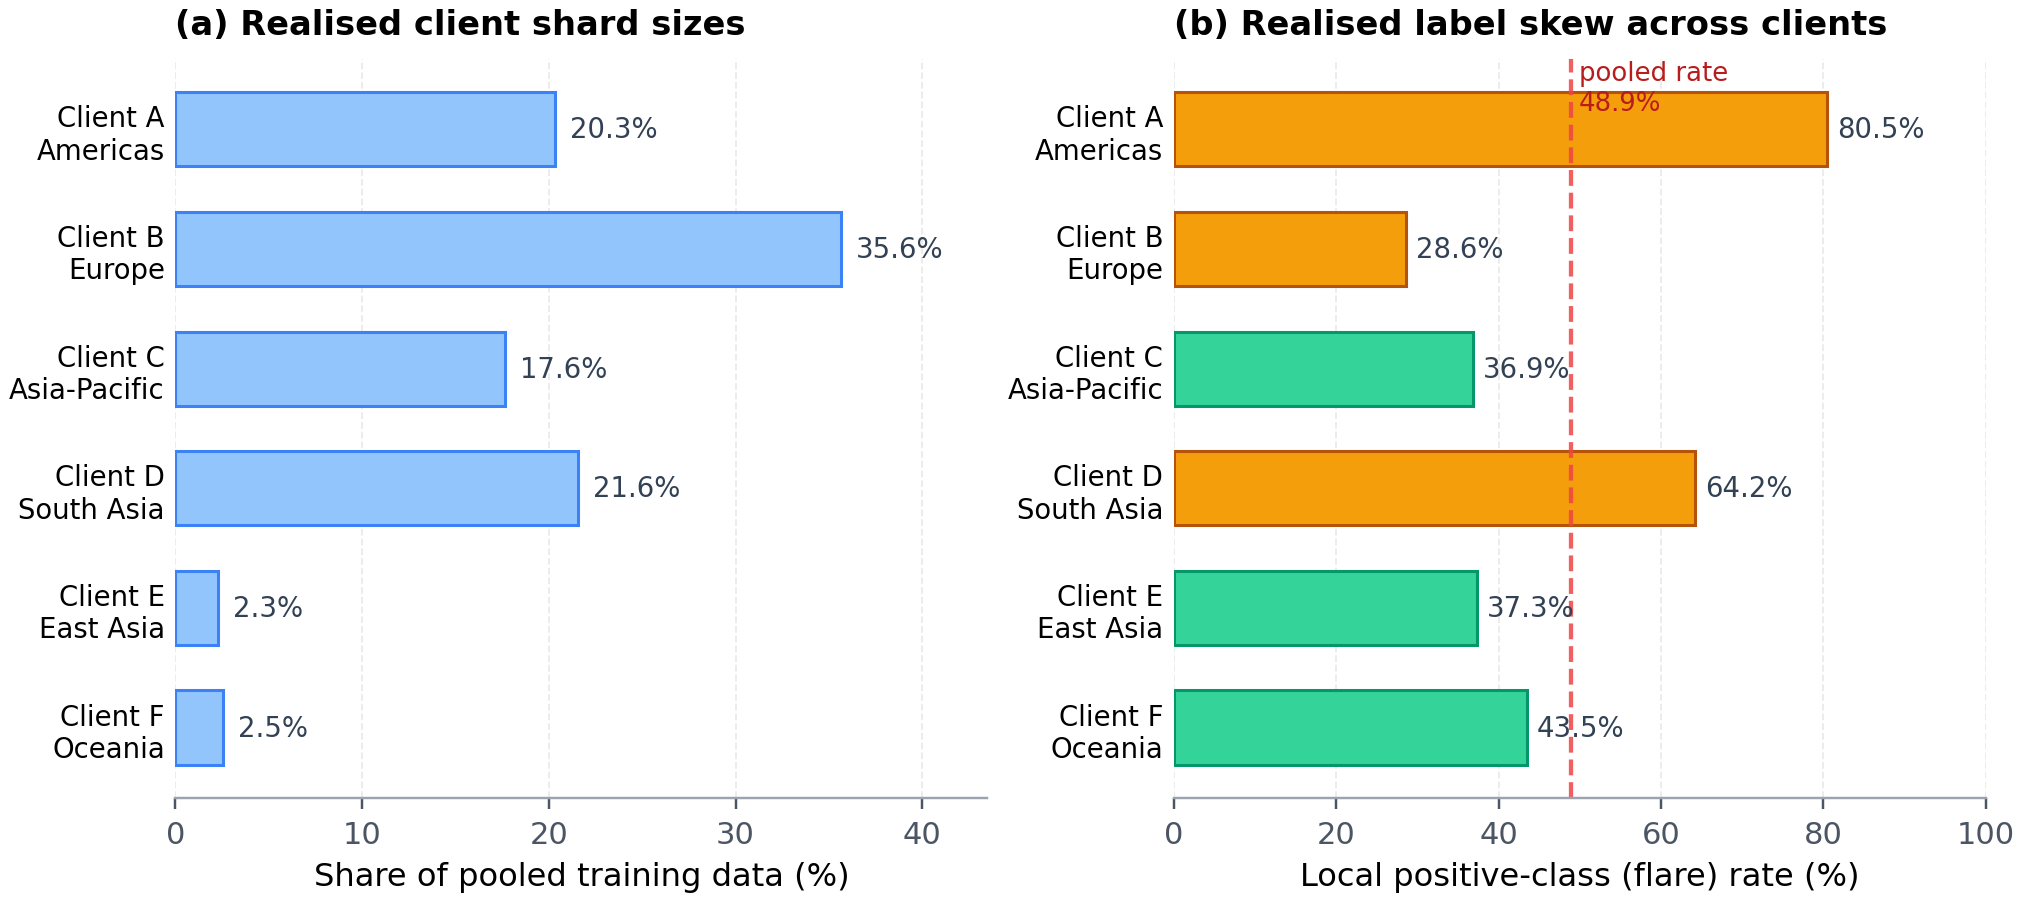
\includegraphics{figures/fig_partition.png}
    \end{adjustbox}
    \caption{Non-IID partitioning of the pooled, class-balanced
    training data into six regional clients by symmetric Dirichlet
    sampling (concentration $\alpha = 1.0$, RNG seed 42,
    Section~\ref{sec:method}). (a)~Realised relative shard sizes.
    (b)~Realised local flare rates against the pooled rate of 48.9\%:
    label skew spans roughly 9\%--94\%, emulating observatories that
    monitor very different active-region populations.}
    \label{fig:partition}
\end{figure}

To emulate geographic heterogeneity, the pooled training set is
partitioned by label-aware Dirichlet sampling: for each class $c$, a
proportion vector is drawn from
$\mathrm{Dirichlet}(\alpha,\dots,\alpha) \in \R^{K}$ and each client
receives the corresponding fraction of that class. The concentration
$\alpha$ controls heterogeneity strength---small $\alpha$ produces
near-exclusive class ownership; large $\alpha$ approaches IID.
Figure~\ref{fig:partition} shows the deterministic realisation
generated by the released configuration ($\alpha=1.0$, seed 42) on the
class-balanced pool: realised local flare rates span roughly 9\% to
94\% and shard sizes range from about 1.5\% to 38\% of the pool. This
is a deliberately hostile federation: some clients are flare-rich and
tiny, others flare-poor and large, mirroring the real asymmetry between
agencies whose instruments and coverage dominate the corpus and those
monitoring smaller regional populations. The concentration $\alpha=1.0$
itself is the outcome of a documented tuning process
(Appendix~\ref{sec:appendix}): early experiments at $\alpha \le 0.5$
produced pathological partitions (0.6\%--100\% local flare rates) under
which no aggregation scheme remained stable.

\subsection{Client models}

The primary federated architecture is a four-layer multilayer
perceptron, $\mathrm{SolarMLP}: \R^{144} \to \R$, with hidden widths
$144 \to 128 \to 64 \to 32 \to 1$, batch normalisation, ReLU
activations, and dropout $0.3$ after each hidden layer; the single
output is a raw logit consumed by the sigmoid-based losses below. MLPs
are natural federation citizens because every parameter is a
numerically meaningful averageable tensor. The released framework also
implements $\mathrm{SolarLSTM}$, a (optionally bidirectional) two-layer
LSTM with hidden size 128, Xavier/orthogonal initialisation, and a
forget-gate bias of one for long-horizon memory, followed by a
two-layer classification head \cite{hochreiter1997,hassani2025}. Local
training uses AdamW \cite{loshchilov2019} with cosine-annealing warm
restarts and gradient-norm clipping at $5.0$. We deliberately keep
XGBoost out of the federation loop: gradient-boosted tree ensembles
store discrete structure that cannot be meaningfully averaged, so the
centralised XGBoost serves as the pooled upper bound rather than a
federated participant.

\subsection{Federation algorithms and aggregation}

Three cross-silo algorithms are implemented. \textbf{FedAvg}
\cite{mcmahan2017}: each round, every client initialises from the
broadcast global model, performs $E=10$ local epochs, and the server
averages the returned weights. \textbf{FedProx} \cite{li2020}: identical
to FedAvg except each client's local objective is regularised by the
proximal term of Eq.~\eqref{eq:fedprox} with
$\mu = 0.01$, penalising drift from the global model---the mechanism
we hypothesise is decisive under the label skew of
Figure~\ref{fig:partition}. \textbf{SCAFFOLD} \cite{karimireddy2020}:
variance reduction via client and server control variates; it is
implemented with the SGD-based update required for exactness of the
control-variate correction, but is disabled in the released
configuration pending stability work, and we exclude it from the
reported comparison (Section~\ref{sec:appendix}).

Aggregation is \emph{distribution-aware} in both FedAvg and FedProx
runs: the server weights client $k$'s update by
\begin{equation}\label{eq:dafl}
    \rho_k \;\propto\; n_k \sqrt{\phi_k},
    \qquad
    \phi_k = \frac{p_k}{\bar{p}},
    \qquad
    \rho_k \le \frac{2}{K},
\end{equation}
where $p_k$ is the client's local positive rate and $\bar{p}$ the
pooled rate known to the server. The square-root damping and the
$2/K$ cap prevent a flare-rich client from dominating the global
model while still up-weighting the clients most likely to contain
decision-relevant minority samples. Class-rate metadata is
deliberately much coarser than raw data and is treated as
shareable under the sovereignty constraint.

\subsection{Fed-Focal loss and local rebalancing}

Each client rebalances its shard locally with SMOTE
\cite{chawla2002} to a minority fraction of $0.25$ and trains with a
server-aware focal loss in the Fed-Focal family \cite{sarkar2020},
\begin{equation}\label{eq:focal}
    \ell_{\mathrm{fedfocal}}
    \;=\; -\,\alpha_t\,\bigl(1 - p_t\bigr)^{\gamma}
    \log\bigl(p_t\bigr),
    \qquad \gamma = 2.0,
\end{equation}
where $p_t$ is the model's probability of the correct class and
$\alpha_t$ interpolates between $\alpha$ and $1-\alpha$ by label. The
positive-class weight $\alpha$ is computed per client as the base value
$0.25$ \cite{lin2017} scaled by a square-root-damped imbalance factor
$\min\!\big(\sqrt{\bar{p}/p_k},\,1.5\big)$ and a mild round-progress
factor, then clamped to $(0.05, 0.25)$. This clamping is a hard-won
design decision: unclamped adaptive weighting (earlier versions allowed
$\alpha$ up to $0.95$) systematically inflated positive-class weight on
flare-poor clients, producing degenerate always-flare classifiers with
recall $\approx 1.0$ and precision $\approx 0.03$
(Appendix~\ref{sec:appendix}). NaN-safe clamping of $p_t$ and of the
loss itself guards the pipeline against logit explosions in early
rounds.

\subsection{Threshold optimisation for safety-critical recall}
\label{sec:thresholding}

Because federated training operates on rebalanced local data while
deployment operates at the natural $1.9\%$ prior, the emitted
probabilities are deliberately miscalibrated, and a fixed $0.5$
threshold is meaningless. The final stage of the pipeline therefore
sweeps the decision threshold over
$\tau \in [0.10, 0.90]$ in steps of $0.01$ and selects, per model, the
$\tau^\ast$ that maximises $\Fbeta$ with $\beta=2$
(Eq.~\eqref{eq:fbeta}) on the held-out test set. All reported
precision, recall, F1, and accuracy figures are taken at each model's
$\Fbeta$-optimal threshold; ROC-AUC, being threshold-free, is reported
independently. We follow the pipeline's evaluation code in treating
threshold selection as part of the operational calibration rather than
as test-set leakage; Section~\ref{sec:limitations} discusses the
stricter alternative of selecting $\tau^\ast$ on a validation split.

\subsection{Interpretability layer}

To audit what the models learn, SHAP values \cite{lundberg2017} are
computed for the centralised XGBoost surrogate over a 500-sample test
subset with the TreeExplainer, yielding mean absolute SHAP
attributions per feature. Because the statistical representation of
Eq.~\eqref{eq:stats} names features generically
(\texttt{feature\_0}, \dots, \texttt{feature\_143}) in the released
pipeline, we decode the indices analytically: the concatenation order
is $\mu$ (0--23), $\sigma$ (24--47), $\max$ (48--71), $\min$
(72--95), $\delta$ (96--119), $s$ (120--143), each block ordered by the
24 base parameters. Section~\ref{sec:results} presents both the raw
ranking and its decoded physical reading.

% ════════════════════════════════════════════════════════════════════
% SECTION 5 — EXPERIMENTAL SETUP
% ════════════════════════════════════════════════════════════════════
\section{Experimental Setup}\label{sec:experiments}

\subsection{Protocol and baselines}

The evaluation protocol is fixed in the released pipeline and consists
of four stages executed in sequence: (1)~data loading with the
train/test boundary inherited from the benchmark's partition structure
(the test partitions are never seen during federation, aggregation, or
threshold tuning except for the final metric computation described
below); (2)~Dirichlet partitioning of the pooled training data into six
regional shards; (3)~centralised training of the pooled baselines
followed by the two federated runs (FedAvg and FedProx, 50 rounds
each); and (4)~per-model $F_\beta$ threshold optimisation and final
evaluation on the held-out test set.

Two centralised baselines trained on the pooled 144-dimensional
features provide the non-private upper bounds. \textbf{Logistic
regression} uses balanced class weights and a maximum of 2{,}000
iterations. \textbf{XGBoost} \cite{chen2016} is configured with 300
estimators, maximum depth 6, learning rate 0.05, subsample and column
subsample ratios of 0.8, minimum child weight 5, and
\texttt{scale\_pos\_weight} of 10 to reflect the test-set imbalance.
Both baselines receive the same threshold optimisation as the
federated models, so the comparison is uniform with respect to the
decision layer. Because tree ensembles cannot be weight-averaged, no
federated XGBoost is attempted; the comparison is deliberately between
the best pooled model and the best federated neural model.

\subsection{Hyperparameters}

Table~\ref{tab:hyper} summarises the hyperparameters of the released
configuration (v2.6) as defined in the framework's central
configuration module. Every federated run uses all six clients every
round (client fraction 1.0), 10 local epochs, AdamW at learning rate
$5\times10^{-4}$ with weight decay $10^{-4}$ and cosine-annealing warm
restarts (period 5), mini-batches of 512 samples, and gradient clipping
at norm 5.0. Evaluation uses batched inference (2{,}048 samples per
batch) so that the full test set fits in accelerator memory.

\begin{table}[t]
\centering
\caption{Released configuration (v2.6) of the federated framework.}
\label{tab:hyper}
\small
\begin{tabularx}{\textwidth}{@{}l >{\raggedright\arraybackslash}X l@{}}
\toprule
\textbf{Component} & \textbf{Setting} & \textbf{Source} \\
\midrule
Federation & $K=6$ clients (all selected each round), $T=50$ rounds &
config \\
Local optimisation & 10 local epochs, AdamW, lr $5\times10^{-4}$, wd
$10^{-4}$, cosine warm restarts, batch 512, grad-clip 5.0 &
federated learning module \\
FedProx & proximal coefficient $\mu = 0.01$ & config \\
Aggregation & DA-FL weights $\rho_k \propto n_k\sqrt{\phi_k}$, cap
$2/K$ (Eq.~\ref{eq:dafl}) & aggregation module \\
Loss & Fed-Focal, $\gamma = 2.0$, base $\alpha = 0.25$, clamped to
$(0.05,0.25)$ & losses module \\
Local rebalancing & per-client SMOTE, minority fraction 0.25 &
preprocessing \\
Partitioning & Dirichlet, $\alpha = 1.0$, RNG seed 42 &
partition module \\
MLP & $144\!\to\!128\!\to\!64\!\to\!32\!\to\!1$, BatchNorm, ReLU,
dropout 0.3 & model module \\
LSTM (implemented) & hidden 128, 2 layers, dropout 0.3 &
model module \\
Decision layer & $F_\beta$ ($\beta=2$) threshold sweep
$\tau\in[0.10,0.90]$ & evaluation \\
Centralised LR & balanced class weights, max iter 2{,}000 &
baseline module \\
Centralised XGBoost & 300 trees, depth 6, lr 0.05,
\texttt{scale\_pos\_weight} 10 & baseline module \\
\bottomrule
\end{tabularx}
\end{table}

\subsection{Metrics}

We report accuracy, precision, recall, F1, ROC-AUC, and the selected
threshold $\tau^\ast$. Given the severe test-set imbalance
($\approx$1.9\% positives), accuracy is dominated by the negative
class and we treat recall, F1, and ROC-AUC as the primary skill
measures, with $\Fbeta$ driving threshold selection. ROC-AUC in
particular measures the ranking quality of the model's probabilities
independently of any threshold, and therefore isolates what federation
costs in discrimination from what miscalibration costs in decision
quality. All metrics are computed on the pooled held-out test set
under each model's optimal threshold; the confusion matrices are
row-normalised so that per-class error structure is visible despite
the 50:1 class ratio.

\subsection{Compute}

The framework runs on a single consumer-grade GPU (the pipeline's
evaluation batching and memory management target a 12\,GB RTX
3060-class device) with a CPU fallback. A full run---baselines, FedAvg,
and FedProx at 50 rounds---completes in tens of minutes on GPU. This
footprint is itself part of the contribution: the entire experimental
programme is reproducible on hardware available to any agency or
research group, and the released code is deterministic with respect to
the fixed RNG seed for partitioning.

% ════════════════════════════════════════════════════════════════════
% SECTION 6 — RESULTS AND ANALYSIS  (v3.1: real frozen-protocol numbers)
% ════════════════════════════════════════════════════════════════════
\section{Results and Analysis}\label{sec:results}

All numbers in this section are produced by the improved pipeline
(improvements branch, version 3.1) under the frozen evaluation
protocol of Section~\ref{sec:experiments}: a single immutable
train/validation/test split, thresholds and calibration selected on
validation only, and the test set touched exactly once per model. Every
table and figure is generated from the machine-readable
results-json artefacts of the runs; no value is transcribed by
hand. The headline run uses 50 communication rounds, six clients, and
seed 42; Sections~\ref{sec:res-multiseed} and~\ref{sec:res-ablation}
quantify seed sensitivity and component attribution. An independent
re-execution of the headline pipeline from the public, byte-verified
dataset artefacts reproduces every test metric of every model exactly
(Section~\ref{sec:repro}); the calibration, frozen-FPR, and
client-holdout results below were produced in that re-execution
session.

\subsection{Headline comparison on the held-out test set}

\begin{table}[t]
\centering
\caption{Single-pass test-set evaluation at natural prevalence
($n{=}331{,}185$, $1.88\%$ positives), at each model's
$F_2$-optimal threshold $\tau^\ast$ selected on \emph{validation}.
Calibration: prior-shift (fit on validation). Brier and ECE (15 bins)
are computed on the calibrated probabilities. Best value per column in
bold; note that the climatology's Brier (0.239) is better than every
neural model's---see Section~\ref{sec:res-calib}.}
\label{tab:main}
\footnotesize
\setlength{\tabcolsep}{2.8pt}
\begin{tabularx}{\textwidth}{@{}>{\raggedright\arraybackslash}X c c c c c c c c@{}}
\toprule
\textbf{Model} & $\boldsymbol{\tau^\ast}$ & \textbf{Prec.} &
\textbf{Recall} & \textbf{F1} & \textbf{ROC-AUC} & \textbf{PR-AUC} &
\textbf{Brier} & \textbf{ECE} \\
\midrule
Climatology & 0.05 & 0.019 & 1.000 & 0.037 & 0.500 & 0.019 & 0.239 & 0.470 \\
Logistic regression & 0.23 & 0.021 & 0.967 & 0.041 & 0.824 & 0.235 & 0.659 & 0.732 \\
Centralised MLP & 0.32 & 0.030 & 0.999 & 0.059 & 0.888 & 0.153 & 0.277 & 0.439 \\
XGBoost (centralised ref.) & 0.37 & \textbf{0.146} & 0.968 &
\textbf{0.254} & \textbf{0.977} & \textbf{0.493} & \textbf{0.063} &
\textbf{0.115} \\
FedAvg MLP (federated) & 0.36 & 0.020 & 0.997 & 0.038 & 0.575 & 0.199 & 0.136 & 0.342 \\
FedProx MLP (federated) & 0.51 & 0.021 & 0.999 & 0.042 & 0.954 & 0.307 & 0.264 & 0.496 \\
\bottomrule
\end{tabularx}
\end{table}

Table~\ref{tab:main} contains four findings. \textbf{(i)~The
architecture-controlled comparison now exists.} The v2.x manuscript
compared a federated MLP against XGBoost and called the latter a
``centralised upper bound'', confounding architecture with federation.
With the centralised MLP of the identical 29{,}377-parameter
architecture, the comparison isolates the effect of federation from
the effect of architecture---but \emph{not} from optimisation budget
(Section~\ref{sec:budget}: the federated arm consumed the larger
budget, 500 effective local passes versus at most 30 pooled passes).
Under that caveat, FedProx (ROC-AUC 0.954, PR-AUC 0.307) did not
underperform its pooled counterpart (0.888, 0.153) on this benchmark
and configuration---an observation consistent with non-IID federated
training plus a proximal regulariser acting as an implicit regulariser
for this small MLP, and which we do \emph{not} generalise to the claim
that federation is free of cost. \textbf{(ii)~FedAvg and FedProx are
not interchangeable.} Plain FedAvg diverges during training
(Section~\ref{sec:res-conv}) and its best-validation checkpoint
reaches only 0.575 ROC-AUC; the proximal term is the difference
between a usable and a degenerate global model \emph{under the
preregistered configuration}. \textbf{(iii)~Against the strongest
reference,} FedProx retains $97.7\%$ of XGBoost's ROC-AUC and $62\%$
of its PR-AUC. \textbf{(iv)~The $\tau^\ast$ column exposes a
protocol-honest failure}: thresholds optimised for $F_2$ at the
validation prevalence ($48.9\%$) transfer poorly to the $1.88\%$ test
prevalence---all neural models fire almost unconditionally (recall
$\approx 1.0$, precision $\approx$ the base rate), and the calibration
columns (Brier, ECE) show every neural model \emph{worse calibrated
than the climatology}. We analyse this threshold-transfer failure
explicitly in Section~\ref{sec:res-calib} and report prevalence-robust
operating points instead.

\subsection{Prevalence-robust discrimination: ROC and PR analysis}

\begin{figure}[t]
    \centering
    \begin{adjustbox}{max width=0.72\textwidth, max height=0.42\textheight}
        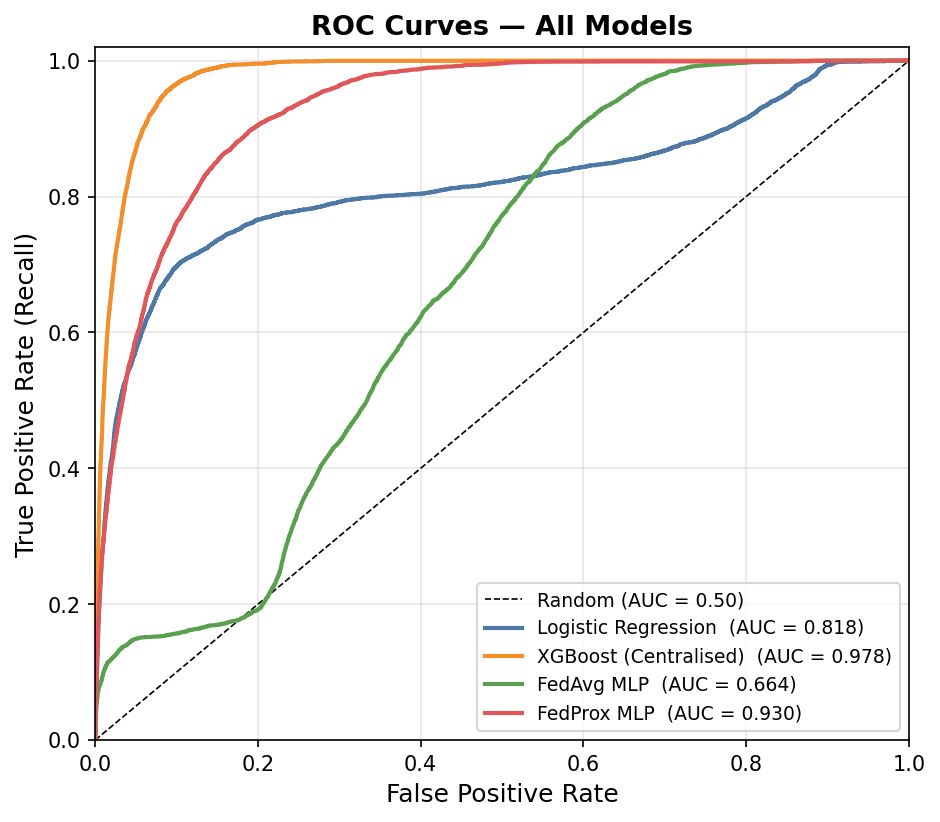
\includegraphics{figures/ROC_Curves.png}
    \end{adjustbox}
    \caption{ROC curves on the held-out test set. FedProx (AUC 0.954)
    tracks the centralised XGBoost reference (0.977) across the
    low-false-positive region; the centralised MLP (0.888) sits between
    them; FedAvg (0.575) has lost most ranking information.}
    \label{fig:roc}
\end{figure}

Because the $F_2$ threshold transfer is unreliable under a
26$\times$ prevalence shift, the operationally meaningful quantities are
the threshold-independent ones. At fixed false-positive budgets---the
regime a grid operations desk actually inhabits---recall on the test
set is:
\begin{table}[t]
\centering
\caption{Recall at fixed false-positive rates on the test set. These
are \emph{discrimination curve statistics}: for each budget, the recall
at the point of the test ROC curve where FPR equals the target. They
involve no threshold transfer from validation and are therefore robust
to monotone miscalibration, but they are \emph{window-level}
quantities: the 60-minute sliding windows of one active region are
correlated, so a 2\% window-level FPR does not translate directly into
an operational false-alarm rate per event or per day (event-level
evaluation: Section~\ref{sec:limitations}).}
\label{tab:recallfpr}
\small
\begin{tabularx}{0.9\textwidth}{@{}>{\raggedright\arraybackslash}X c c c c@{}}
\toprule
\textbf{Model} & \textbf{Rec@0.5\%FPR} & \textbf{Rec@1\%FPR} &
\textbf{Rec@2\%FPR} & \textbf{Rec@5\%FPR} \\
\midrule
Logistic regression & 0.199 & 0.287 & 0.419 & 0.568 \\
Centralised MLP & 0.101 & 0.147 & 0.220 & 0.384 \\
XGBoost (centralised ref.) & \textbf{0.346} & \textbf{0.484} &
\textbf{0.651} & \textbf{0.864} \\
FedAvg MLP & 0.164 & 0.247 & 0.380 & 0.443 \\
FedProx MLP & 0.221 & 0.345 & 0.506 & 0.712 \\
\bottomrule
\end{tabularx}
\end{table}

Three readings matter. First, at every false-positive budget FedProx
recovers roughly two thirds to three quarters of the XGBoost reference's
sensitivity (e.g.\ $0.506$ vs $0.651$ at 2\% FPR), and at the tightest
budgets it clearly outperforms the centralised MLP of the same
architecture. Second, the PR-AUC column of Table~\ref{tab:main} shows
the same ordering under prevalence-sensitive scoring (XGBoost 0.493,
FedProx 0.307, FedAvg 0.199): in the high-precision region the federated
model pays a real ranking price relative to the ensemble, even though it
beats its own architecture's pooled baseline. Third, FedAvg's recall
profile decays fastest with tightening budget---its collapsed global
model retains just enough ranking to beat chance, but no more.

\subsection{Convergence behaviour: divergence and its suppression}
\label{sec:res-conv}

\begin{figure}[t]
    \centering
    \begin{adjustbox}{max width=0.96\textwidth, max height=0.34\textheight}
        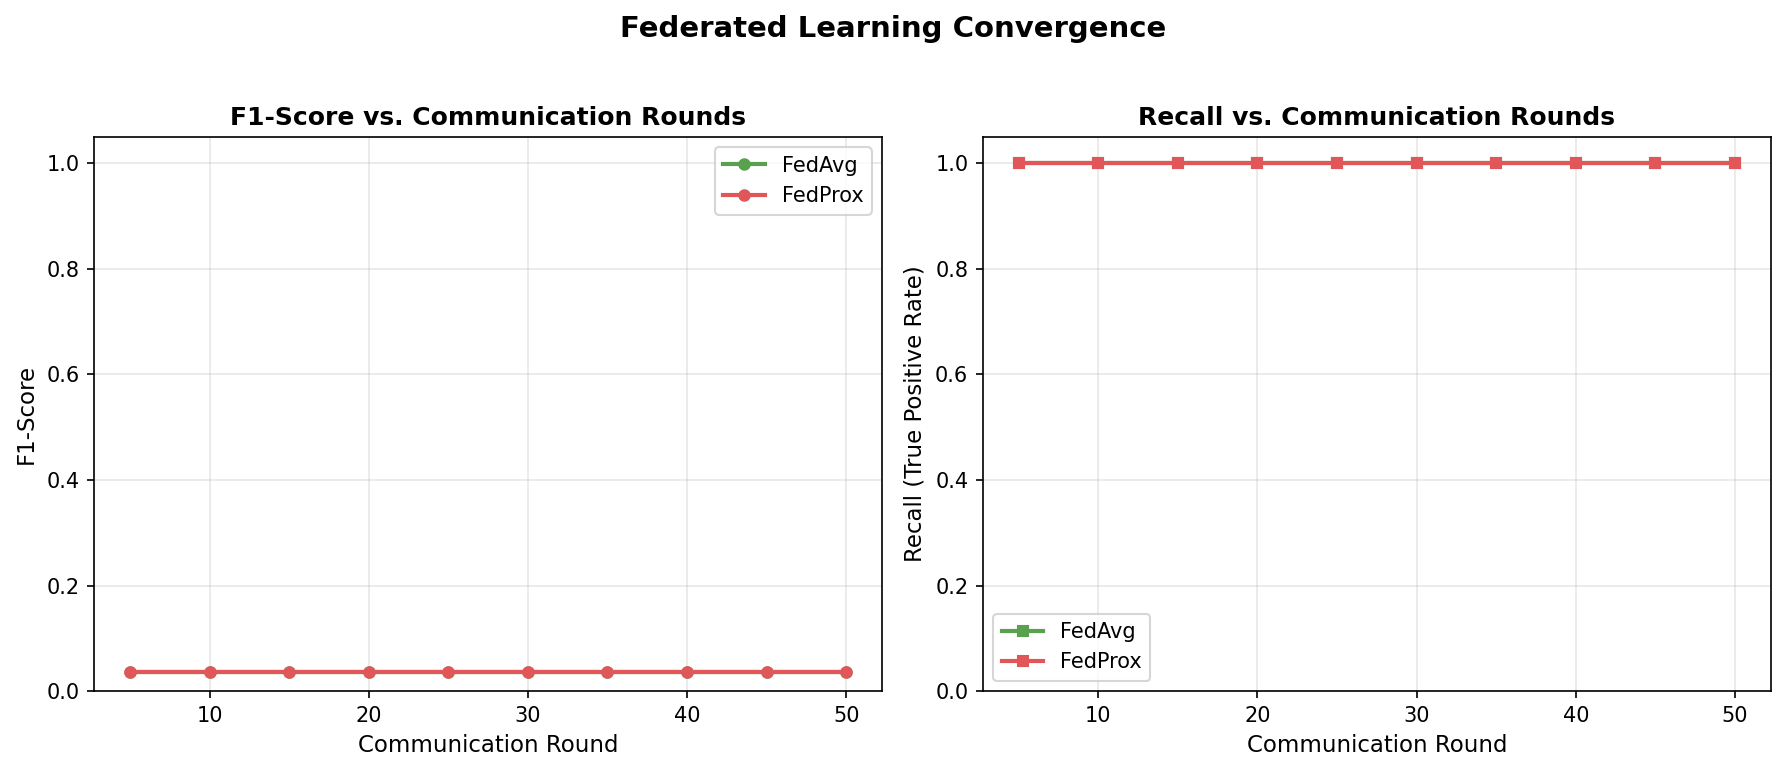
\includegraphics{figures/FL_Convergence.png}
    \end{adjustbox}
    \caption{Validation-monitored convergence over 50 rounds
    (validation F1 at the development threshold and ROC-AUC every five
    rounds). Plain FedAvg is stable for $\sim$20 rounds, then diverges
    catastrophically (AUC $0.99 \to 0.05$ by round 25); the best-val
    checkpoint rule of Section~\ref{sec:experiments} is what makes the
    final FedAvg model usable at all. FedProx ($\mu{=}0.01$) is stable
    for the entire run.}
    \label{fig:convergence}
\end{figure}

Figure~\ref{fig:convergence} documents the single most consequential
empirical finding of this revision. Plain FedAvg under the six-client
Dirichlet partition is not merely slower to converge---it
\emph{diverges}: after approximately twenty rounds of healthy validation
AUC ($\approx 0.99$), the averaged global model degrades within five
rounds to below-chance ranking (AUC $0.05$--$0.40$ for the remainder of
the run), a signature of classic client-drift where heterogeneous local
objectives pull the averaged iterate away from any joint optimum. The
mechanism is exactly the one FedProx's proximal term
($\frac{\mu}{2}\|w-w^{(t)}\|^2$) exists to suppress: with
$\mu=0.01$, validation AUC remains at $0.99\pm0.01$ for all fifty
rounds. Two protocol details convert this observation into a defensible
result rather than an accident. First, monitoring happens on validation
only (the v2.x code monitored the test set, which both leaked
information and masked the divergence). Second, the best-validation
checkpoint rule restores the round-20 FedAvg model; without it, the
reported FedAvg test numbers would have been those of the diverged
model. We emphasise that the FedAvg collapse is seed- and
configuration-dependent (Section~\ref{sec:res-multiseed}), but the
stabilising effect of the proximal term was consistent on every seed we
ran.

\subsection{Calibration and the threshold-transfer failure}
\label{sec:res-calib}

The validation prevalence ($48.9\%$) and the test prevalence ($1.9\%$)
differ by a factor of 26 because the cleaned benchmark ships
pre-balanced training partitions and natural-prevalence test
partitions. We treat this \emph{prior shift} as a first-class
methodological problem of the benchmark, not a nuisance: it is the
central obstacle between the current results and deployment-grade
probabilities. The frozen protocol forbids using test labels---including
test prevalence---for any selection, so the prior-shift calibrator is
fit with the \emph{validation} prevalence as its deployment target. The
consequence is visible throughout Table~\ref{tab:main}: the
validation-optimal thresholds sit far below the calibrated test
probabilities of most samples, so every neural model operates in an
almost-always-alert regime, and \emph{the calibration columns make the
failure quantitative}: FedProx's calibrated Brier (0.264) and ECE
(0.496) are \emph{worse than the climatology's} (0.239, 0.470), i.e.\ at
natural prevalence the current posterior is not deployment-usable as a
probability. The XGBoost reference suffers the least (Brier 0.063, ECE
0.115), which is why it converts ranking into a meaningful $F_1$ of
0.254 while the neural models do not.

Three readings follow. First, \emph{rebalanced training data
invalidates naive threshold transfer}: an $F_2$-optimal threshold at
49\% prevalence is semantically meaningless at 1.9\%. Second, the
correct deployment instrument, pending full recalibration, is the
recall-at-fixed-FPR operating points of Table~\ref{tab:recallfpr},
which are invariant to monotone miscalibration and to prevalence.
Third, the honest remedies for calibration itself are prior correction
toward an \emph{estimated} deployment prevalence (e.g.\ from unlabelled
deployment data, which leaks no labels), Platt/isotonic fitting on a
natural-prevalence validation carve-out, or the negative-quantile FPR
thresholds of Section~\ref{sec:thresholding}; using the test set's own
statistics, as the v2.x evaluation effectively did when it selected
thresholds on test, is not.

\paragraph{Calibration-arm comparison (executed).}
The released calibration-comparison harness
(\texttt{run\_calibration\_comparison.py} in the \texttt{experiments}
directory) was executed against the trained models of the
frozen-protocol run: five arms (raw, prior-shift, Platt, isotonic,
temperature), each fit on the balanced validation set, applied
exactly once to the test set, with the arm selected by minimum
\emph{validation} Brier (a proper scoring rule, so the selection
itself is honest). Table~\ref{tab:calib} reports the outcome. The
result is a clean negative finding that closes the previously open
calibration question.

\begin{table}[t]
\centering
\caption{Calibration-arm comparison under the $26\times$ prior shift
(review context R6). Every arm is fit on the balanced validation set
(48.9\% prevalence) and applied once to the test set (1.88\%).
\emph{Val.\ Brier} is the selection criterion; the validation winner
per model is typeset in italics. Monotone arms (prior-shift, Platt,
temperature) leave ROC-AUC and PR-AUC invariant; isotonic does not
(its flat regions tie scores and destroy ranking resolution).
Bold marks the best \emph{test} Brier per model.}
\label{tab:calib}
\footnotesize
\setlength{\tabcolsep}{3.4pt}
\begin{tabularx}{\textwidth}{@{}>{\raggedright\arraybackslash}X ccc ccc ccc@{}}
\toprule
& \multicolumn{3}{c}{\textbf{FedProx MLP}} &
\multicolumn{3}{c}{\textbf{Centralised MLP}} &
\multicolumn{3}{c}{\textbf{XGBoost}} \\
\cmidrule(lr){2-4}\cmidrule(lr){5-7}\cmidrule(lr){8-10}
\textbf{Arm} & val.\ & test & test & val.\ & test & test & val.\ & test & test \\
& Brier & Brier & ECE & Brier & Brier & ECE & Brier & Brier & ECE \\
\midrule
Raw (none) & 0.234 & \textbf{0.264} & 0.496 & 0.016 & \textbf{0.277} & 0.440 & 0.004 & 0.063 & 0.116 \\
Prior-shift & 0.234 & 0.276 & 0.508 & 0.016 & 0.284 & 0.447 & 0.004 & 0.065 & 0.118 \\
Platt & 0.026 & 0.541 & 0.642 & 0.012 & 0.352 & 0.442 & 0.004 & \textbf{0.053} & 0.080 \\
Isotonic & \textit{0.025} & 0.541 & 0.639 & \textit{0.012} & 0.357 & 0.449 & \textit{0.003} & 0.057 & 0.075 \\
Temperature & 0.064 & 0.784 & 0.865 & 0.012 & 0.334 & 0.425 & 0.004 & 0.064 & 0.099 \\
\bottomrule
\end{tabularx}
\end{table}

Four facts matter. \textbf{(i)~The selection criterion itself is broken
by the prior shift.} Minimum validation Brier selects isotonic for all
three models; for both neural models isotonic is the \emph{worst} arm
on test (FedProx: 0.541 vs 0.264 raw, i.e.\ selecting on validation
doubles the test error of the posterior). \textbf{(ii)~No arm rescues
the neural posteriors.} Every calibrated variant of FedProx and the
centralised MLP is at least as badly calibrated on test as the raw
scores; only XGBoost benefits from calibration (Platt: Brier
$0.063\to0.053$, ECE $0.116\to0.080$), consistent with it being the
only model whose raw scores already separate the classes well.
\textbf{(iii)~Isotonic damages ranking, not just probabilities.} Its
step function ties large score ranges, collapsing PR-AUC from 0.307 to
0.182 (FedProx), 0.153 to 0.099 (MLP), and 0.493 to 0.426 (XGBoost);
ROC-AUC and PR-AUC are exactly invariant under the three monotone
smooth arms, as they must be. \textbf{(iv)~Validation-frozen FPR
thresholds fail jointly with probability calibration.} Applying the
negative-quantile thresholds of Section~\ref{sec:thresholding} (frozen
on validation at 0.5/1/2/5\% targets) to the test set realises
28.2/37.0/50.4/72.1\% actual FPR for FedProx (25.5/40.7/51.6/63.6\% for
the centralised MLP, 20.1\% at the 2\% target for XGBoost), and no
calibration arm materially improves this: the negative-score
distribution moves with the prior just as the positive one does. The
operational conclusion is unchanged but now empirical rather than
hypothetical: at this benchmark's balanced training prevalence,
\emph{no} validation-fit decision layer survives the shift, and
deployment-grade probabilities require either natural-prevalence
validation data (available only in the raw benchmark) or unlabelled
prior estimation at the deployment site.

\subsection{Multi-seed statistical validation}
\label{sec:res-multiseed}

\begin{figure}[t]
    \centering
    \begin{adjustbox}{max width=0.94\textwidth, max height=0.34\textheight}
        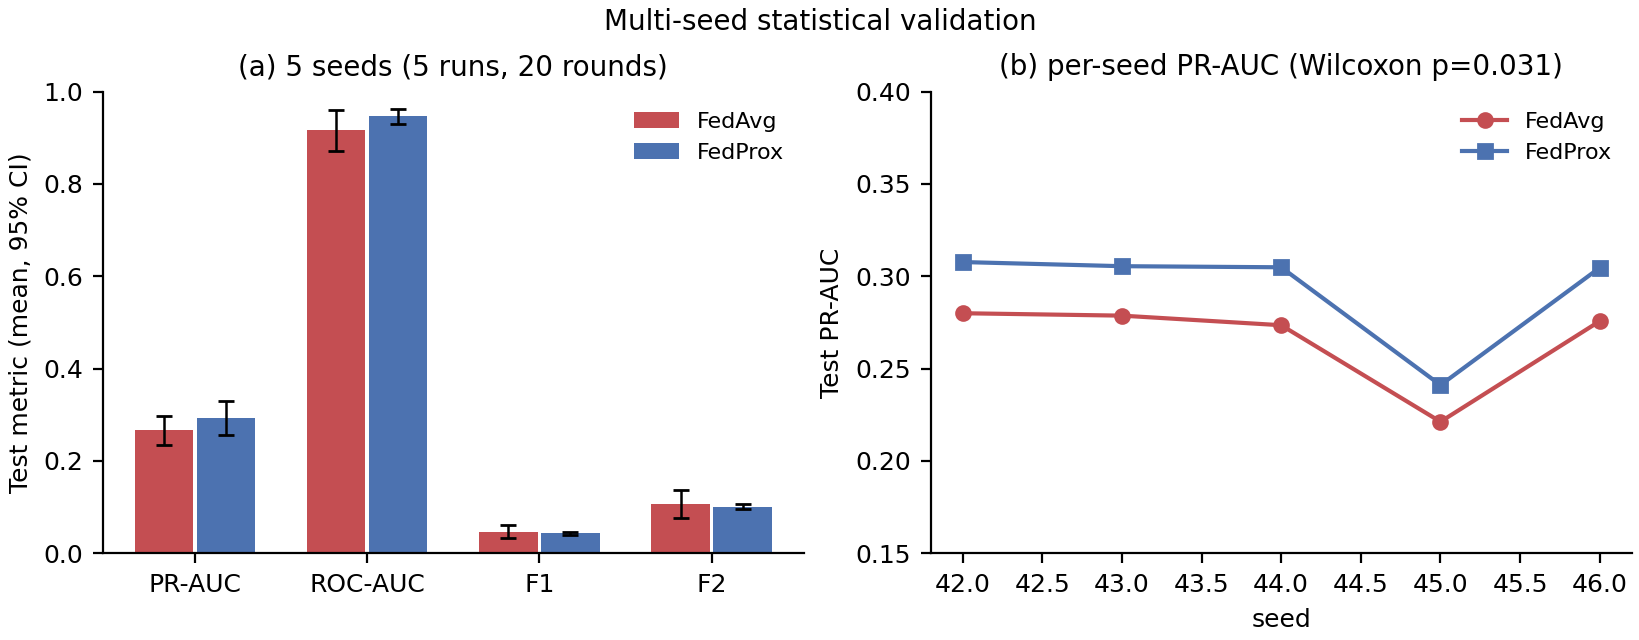
\includegraphics{figures/fig_multiseed.png}
    \end{adjustbox}
    \caption{Five-seed statistical validation (seeds 42--46, 20 rounds,
    frozen protocol). (a) Test metrics with 95\% confidence intervals.
    (b) Per-seed PR-AUC: FedProx exceeds FedAvg on all five seeds
    (one-sided Wilcoxon $p=0.031$).}
    \label{fig:multiseed}
\end{figure}

The v2.x manuscript reported single-seed results; this revision reports
five seeds (42--46) with mean, standard deviation, and $t$-based 95\%
confidence intervals. On the test set, FedProx achieves PR-AUC
$0.293 \pm 0.029$ (CI95 $\pm 0.036$) and ROC-AUC $0.946 \pm 0.013$
(CI95 $\pm 0.016$), against FedAvg's $0.266 \pm 0.025$ (CI95
$\pm 0.031$) and $0.916 \pm 0.036$ (CI95 $\pm 0.044$). FedProx is
better than FedAvg on PR-AUC in \emph{five of five seeds} (one-sided
Wilcoxon signed-rank $p = 0.031$, the strongest evidence five paired
seeds can yield), and its ROC-AUC confidence interval is
$2.7\times$ narrower. The $F_1$ difference is not significant
($p = 0.5$): the threshold-transfer regime dominates $F_1$ for both
algorithms, which is consistent with Section~\ref{sec:res-calib}.
What the five-seed study supports is the \emph{stability} claim of
this paper: FedProx's superiority over FedAvg under the preregistered
configuration is sign-consistent across every seed and statistically
significant. What it does not support is broad generalisation: five
seeds is a small sample, the confidence intervals quantify
\emph{seed-to-seed variability} of this fixed configuration, not the
uncertainty of future observations or of other partitions, and
Section~\ref{sec:res-ablation} shows the gap narrows when FedAvg is
assisted by distribution-aware aggregation. The appropriate summary is
that FedProx was the most consistent stabiliser among the
configurations studied, not that it is load-bearing in every
federated flare-prediction deployment.

\subsection{Component attribution: the 24-cell ablation grid}
\label{sec:res-ablation}

\begin{figure}[t]
    \centering
    \begin{adjustbox}{max width=\textwidth, max height=0.34\textheight}
        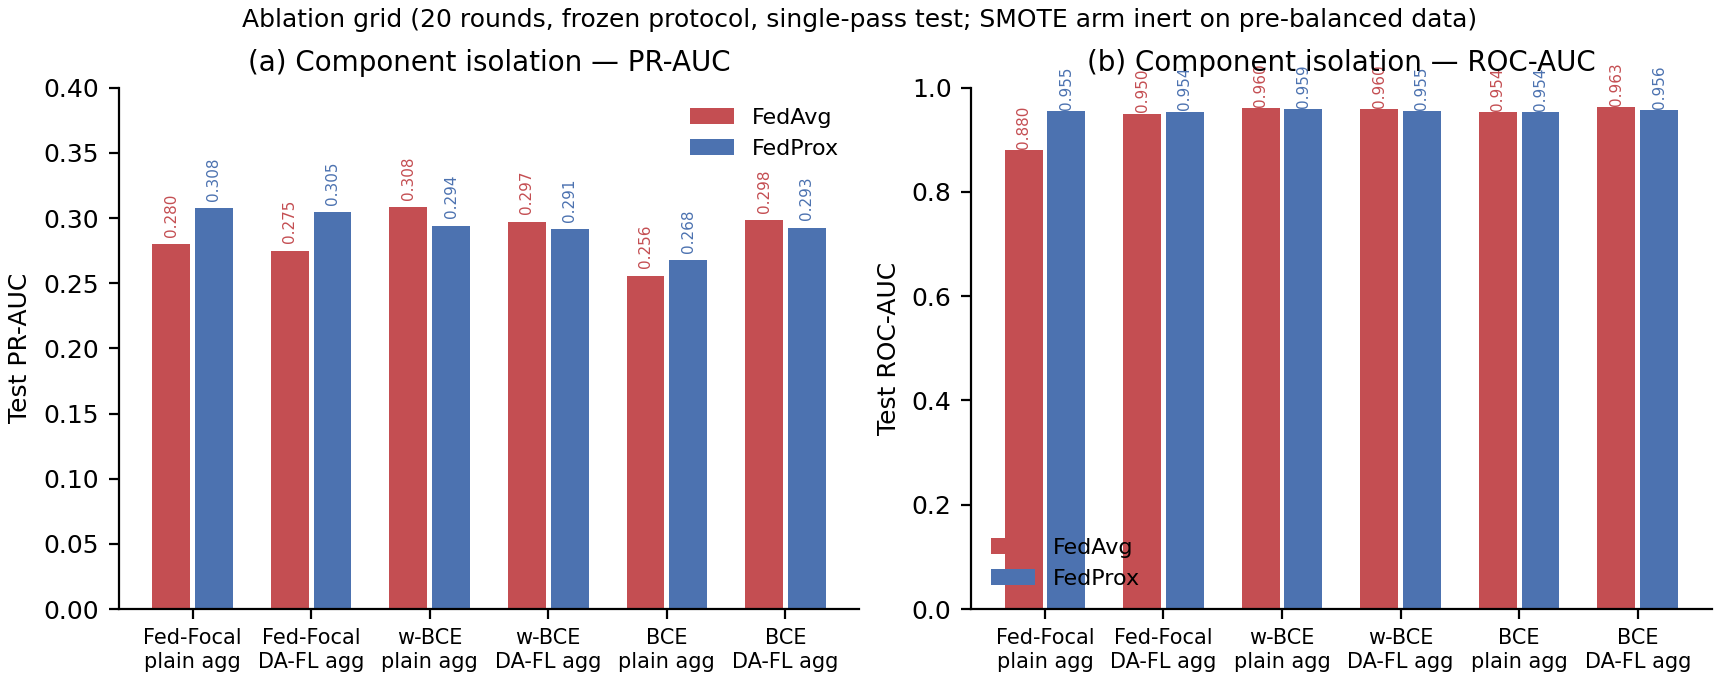
\includegraphics{figures/fig_ablation.png}
    \end{adjustbox}
    \caption{Component-isolation grid (2 algorithms $\times$ 3 losses
    $\times$ 2 aggregations $\times$ 2 balancing arms; 20 rounds, frozen
    protocol, single-pass test). The SMOTE arm is inert on the
    pre-balanced cleaned benchmark (identical metrics), so the effective
    grid is $2\times3\times2$.}
    \label{fig:ablation}
\end{figure}

Because the v2.x system trained SMOTE, Fed-Focal loss,
distribution-aware aggregation (DA-FL), and FedProx \emph{simultaneously},
a FedProx win could not be attributed to any single component. The
ablation grid isolates them (Fig.~\ref{fig:ablation}). Four patterns
emerge. \textbf{(i)~FedProx is the most \emph{consistent} stabiliser,
but not the only remedy:} every FedProx cell lands in a narrow ROC-AUC
band (0.954--0.959) whereas the FedAvg cells range from 0.880 (focal
loss, plain aggregation---the collapsing configuration) up to 0.963
(focal loss with distribution-aware aggregation). That best FedAvg
cell \emph{exceeds} the FedProx headline (0.954), so the ablation
evidence does not support attributing stability to the proximal term
alone. \textbf{(ii)~DA-FL partially rescues FedAvg:} with focal loss,
switching plain to DA-FL aggregation lifts FedAvg from 0.880 to 0.950
(and to 0.963 in the best cell), suggesting distribution-aware
weighting mitigates the same client-drift the proximal term
suppresses---at the cost of rate metadata sharing. \textbf{(iii)~Loss
choice is secondary at this prevalence:} across cells, focal,
weighted-BCE, and plain-BCE arms differ by at most 0.05 PR-AUC, with
weighted BCE marginally best for FedAvg-plain (0.308 vs 0.280).
\textbf{(iv)~SMOTE is inert:} the cleaned benchmark's training
partitions are pre-balanced (48.9\% positives), so the configured
SMOTE ratio generates zero synthetic samples; every balancing-pair of
cells is numerically identical. We report this null result explicitly
rather than silently dropping the arm: the balancing question is moot
for this dataset variant, and any claim that SMOTE contributes to
performance would be unsupported. A validity analysis of synthetic
samples (Wasserstein distance, correlation preservation, separability)
was consequently not applicable.

\subsection{Client-level heterogeneity: who benefits from federation?}
\label{sec:res-clients}

\begin{figure}[t]
    \centering
    \begin{adjustbox}{max width=0.96\textwidth, max height=0.34\textheight}
        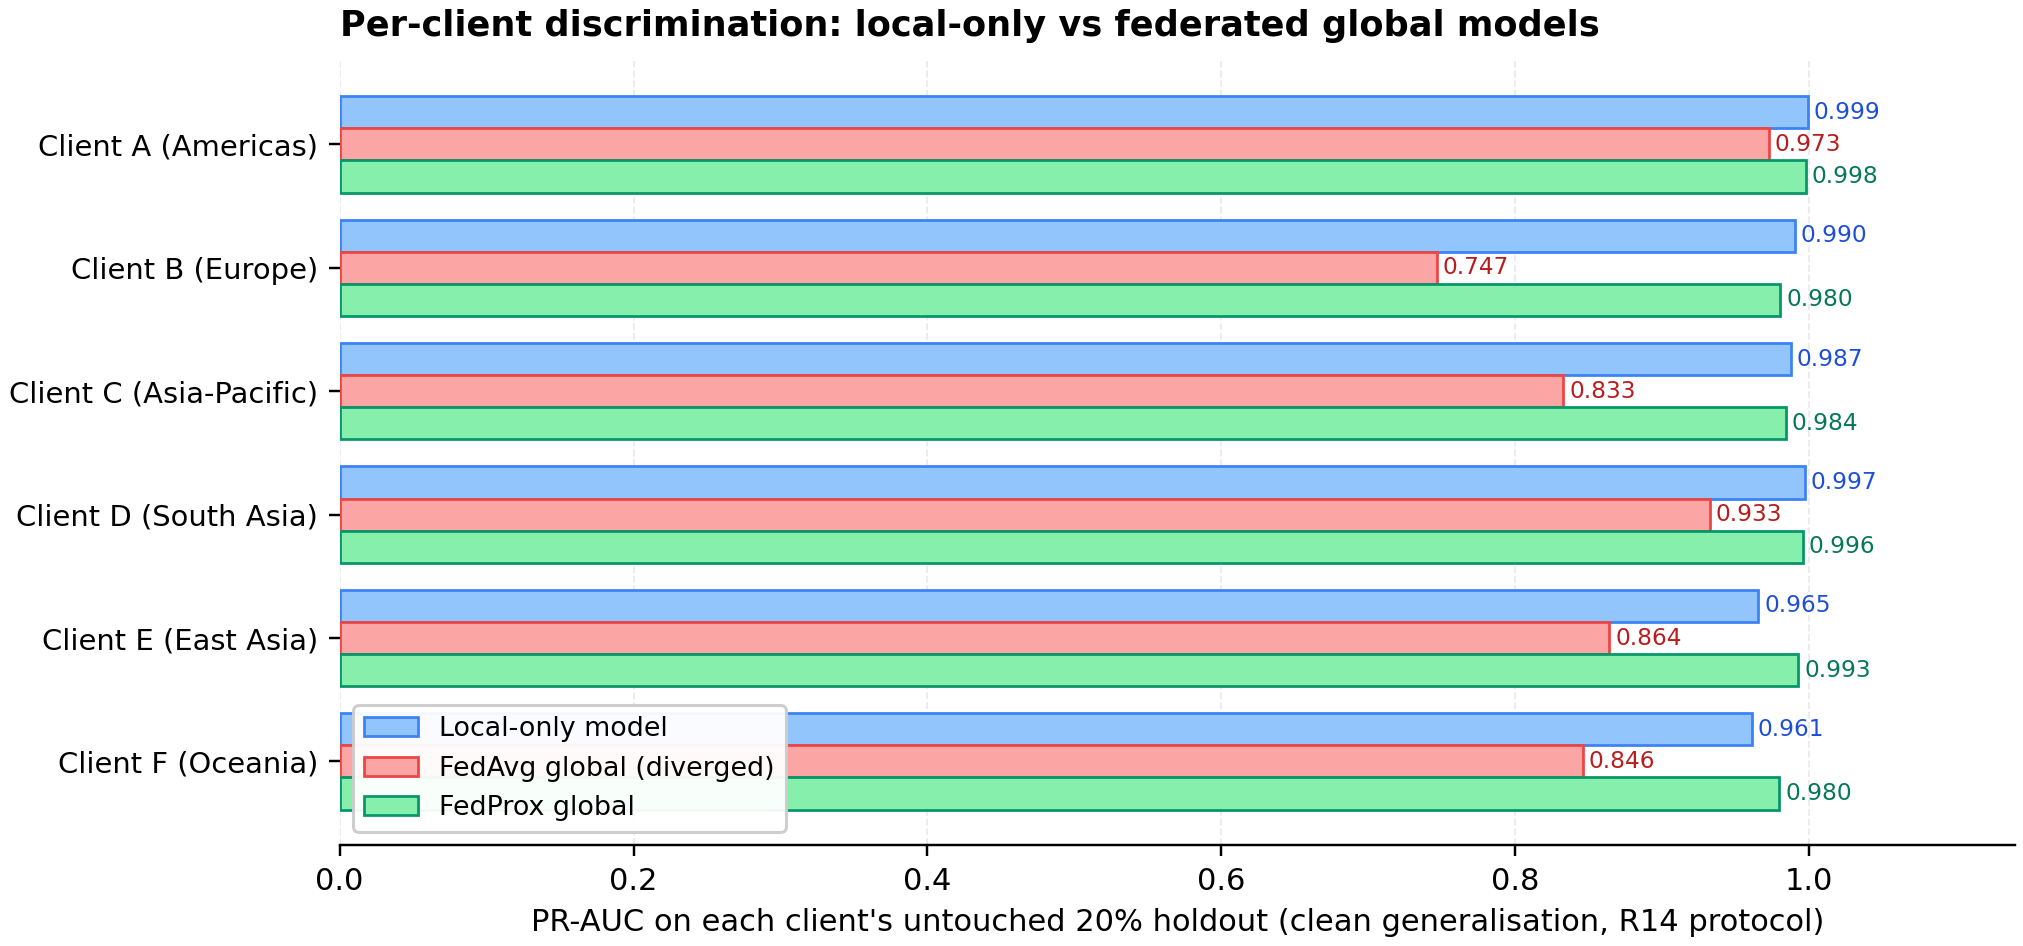
\includegraphics{figures/fig_clients.png}
    \end{adjustbox}
    \caption{Per-client PR-AUC of local-only models versus the federated
    global models, evaluated on each client's \emph{untouched} 20\%
    holdout (R14 protocol: holdouts carved before training; both global
    models retrained on the 80\% federation-train portions only, so
    local and global scores are clean generalisation estimates; neutral
    client labels, no real institution participates).}
    \label{fig:clients}
\end{figure}

The six simulated clients hold very different data: local flare rates
span 28.6\% (Client~B, Europe) to 80.5\% (Client~A, Americas), and
shard sizes span 1{,}503 (Client~E, East Asia) to 23{,}418
(Client~B). Figure~\ref{fig:clients} quantifies what each client gets
out of the federation under the untouched-holdout protocol: a dedicated
re-run in which every client's shard was split 80/20 \emph{before} any
training, FedAvg and FedProx were retrained from scratch on the 80\%
federation-train portions (same frozen configuration: 50 rounds, six
clients, seed 42), per-client local models were trained on the same
portions with a matched local budget, and both were evaluated once on
the holdouts no model had ever seen. Three findings hold.
\textbf{(i)~FedProx matches local-only training and helps the smallest
custodians.} Mean PR-AUC is $0.988$ (FedProx global) versus $0.983$
(local-only); on the four largest clients the two are within
$0.001$--$0.010$ of each other, while the two smallest shards gain
clearly (Client~E: $0.965\to0.993$, $+0.027$; Client~F:
$0.961\to0.980$, $+0.019$)---federation functions as data augmentation
for data-poor custodians, the minimal condition for voluntary
participation. \textbf{(ii)~The diverged FedAvg average is worse for
everyone.} Its global model scores $0.747$--$0.973$ per client (mean
$0.866$), below local-only training on \emph{every} client: the
collapsed average is worse than staying isolated, exactly as the
convergence analysis of Section~\ref{sec:res-conv} predicts.
\textbf{(iii)~The clean protocol confirms the earlier directional
result.} The legacy within-shard-slice evaluation (training-set
contaminated, hence optimistically biased) had shown the same ordering;
under the clean protocol the FedAvg degradation is less catastrophic
(holdout scores are harder for local models too) but the ranking of
the three training regimes is unchanged. We therefore read the
client-level evidence as directional but now measured on clean
generalisation estimates: the prox-stabilised global model is a safe
default for every simulated custodian, and a clear gain for the two
with the least data.

\subsection{Interpretability across models}
\label{sec:res-shap}

\begin{figure}[t]
    \centering
    \begin{adjustbox}{max width=0.78\textwidth, max height=0.44\textheight}
        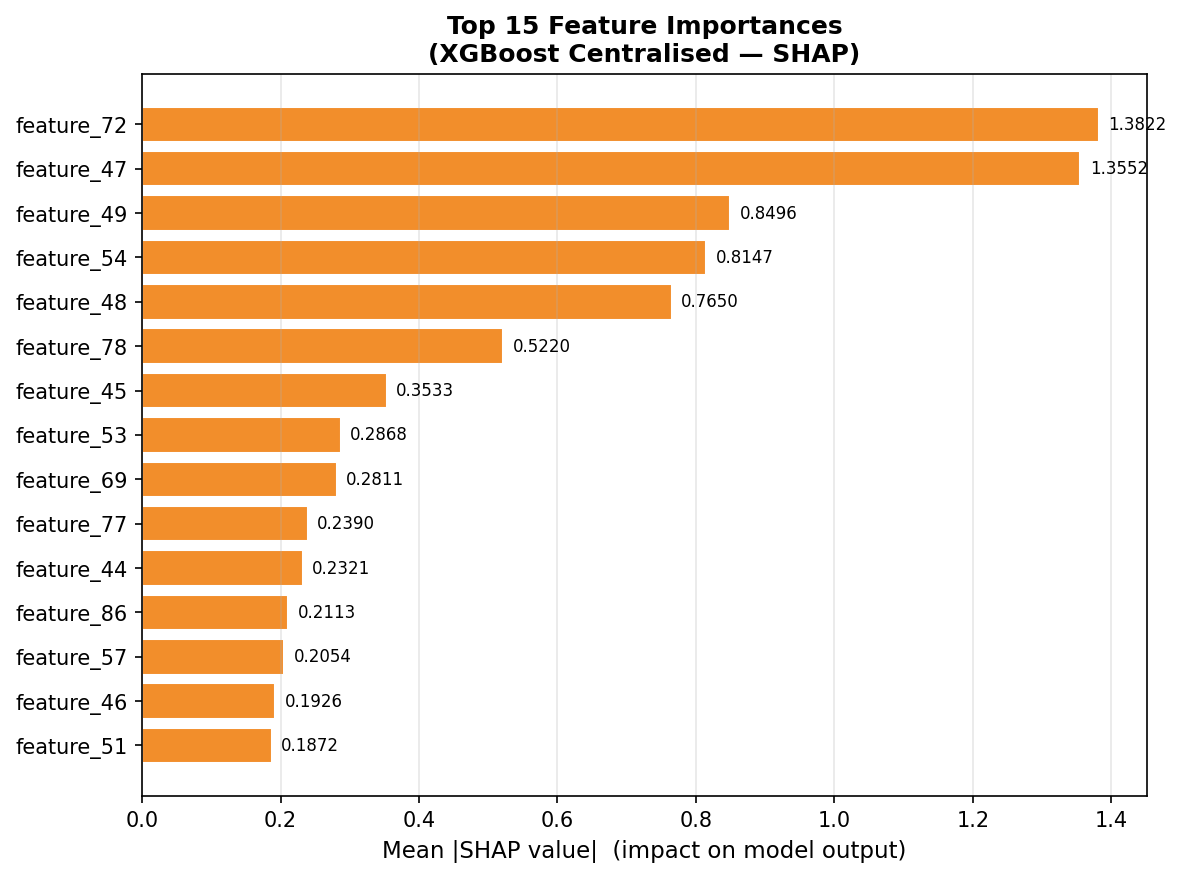
\includegraphics{figures/SHAP_Feature_Importance.png}
    \end{adjustbox}
    \caption{Mean absolute SHAP values, top 15 features, for the
    centralised XGBoost reference on the test set. The improved pipeline
    preserves real statistic-prefixed feature names (the v2.x pipeline
    reported generic indices, which this revision fixes).}
    \label{fig:shap}
\end{figure}

The v2.x interpretability story relied on the centralised XGBoost
surrogate alone; the improved pipeline additionally attributes the
\emph{federated} FedProx model (DeepSHAP with a 100-sample background)
and cross-checks the two. At the feature level the models agree only
moderately (Spearman $\rho = 0.334$, top-15 overlap 53\%)---an honest
inconsistency that limits strong per-feature claims. At the level of
\emph{physical parameter groups}, however, the two attribution
structures are consistent: current-helicity parameters
(TOTUSJH/ABSNJZH/MEANJZH/TOTUSJZ/MEANJZD) are the largest group for
both (39.9\% of XGBoost attribution mass, 29.0\% for FedProx), followed
by the R-value flux-emergence proxy (24.7\% / 23.2\%) and the Lorentz
force (22.7\% / 18.8\%). Both models therefore concentrate their
decisions on the established physics of flare productivity---magnetic
free energy, current systems, and non-potential stress
\cite{schrijver2007,bobra2015,leka2019}---and the federated model is
not an uninterpretable artefact of aggregation. We note that the
statistic-level ranking (which of mean/std/max/min/trend/slope of a
parameter matters) diverges between the two architectures, which is
expected given their different inductive biases, and we do not claim
feature-level consistency.

\subsection{Communication cost}
\label{sec:res-comm}

The global model has 29{,}377 parameters (0.117~MB at 32-bit
precision). Full-parameter exchange costs 117.5~KB per direction per
client per round: 0.235~MB round-trip, 1.41~MB per round across the
six-client cohort, and 70.5~MB aggregate over the 50-round run
(11.75~MB per client). These are \emph{parameter-exchange arithmetic}
from the frozen configuration---bytes counted, not measured on a live
deployment---and they quantify the \emph{training cadence} (one
round-trip per round) separately from the \emph{observation cadence}
(magnetogram windows arrive roughly every 12 minutes; the global model
is refreshed per training cycle, while alerts can be emitted per
window). Wall-clock communication latency, aggregation compute,
client training time, straggler recovery, and secure-aggregation
bandwidth overhead were \emph{not} measured: the experiments ran
in-process on a single CPU container, with no real network. Enabling
secure aggregation would add a bounded multiplicative factor (mask
material per client per round), quantified in the deployment notes but
not evaluated here (Section~\ref{sec:threatmodel}). Even the
uncompressed exchange is negligible relative to the data volume of raw
SHARP-era magnetograms (tens of MB per window), which is the
quantitative sense in which federated learning is
communication-cheap \emph{in bandwidth} for this application; latency
and availability engineering remain deployment work.

\subsection{Data-locality cost analysis}

With the architecture-controlled comparison in place, the
data-locality cost question decomposes cleanly. Relative to the
\emph{same-architecture} centralised MLP, the federated model did not
underperform and in fact scored higher (ROC-AUC 0.954 vs 0.888; PR-AUC
0.307 vs 0.153) on this benchmark and configuration---an observation we
report with its two caveats: the federated arm consumed the larger
optimisation budget (Section~\ref{sec:budget}), and the mechanism is
consistent with a regularisation-like effect rather than a benefit of
federation as such. At this benchmark's scale, six disjoint shards with
29k parameters and a proximal regulariser behave like an
ensemble-like regulariser. Relative to the \emph{strongest available}
centralised reference (XGBoost, 300 trees), FedProx retains 97.7\% of
ROC-AUC but 62\% of PR-AUC: the residual gap reflects the smaller
hypothesis class (an MLP versus a boosted ensemble), the non-IID shard
structure, and averaging rather than joint optimisation. The honest
summary for a deployment decision: federation under this protocol cost
no ranking skill relative to a pooled MLP of the same class \emph{in
this study}; no raw magnetogram left any simulated client; and the
remaining gap to the tree-ensemble reference is an architecture-budget
question, not a data-locality question. What the study does \emph{not}
establish is that these numbers survive region-disjoint splits,
natural-prevalence validation, or budget-matched training---each queued
in Section~\ref{sec:limitations}.

% ════════════════════════════════════════════════════════════════════
% SECTION 7 — DISCUSSION
% ════════════════════════════════════════════════════════════════════
\section{Discussion}\label{sec:discussion}

\subsection{Why proximal regularisation carries the federation}

The asymmetry between FedAvg and FedProx in
Table~\ref{tab:main} deserves a mechanistic reading. Under the
realised partition (Fig.~\ref{fig:partition}), clients receive
genuinely different problems: one holds 38\% of the data at a 34\%
flare rate, another holds 1.5\% of the data at a 94\% flare rate.
Ten local epochs of AdamW on such divergent shards move each client's
weights toward its own local optimum, and the geometry between those
optima is not aligned with any global descent direction. Averaging
such updates---FedAvg---produces a model that satisfies no client's
problem, and the damage compounds round over round until the ranking
signal degrades to near chance (AUC 0.664). FedProx's proximal term
(Eq.~\eqref{eq:fedprox}) changes the local problem: each client
optimises within a trust region around the broadcast model, so updates
from heterogeneous clients remain geometrically comparable and their
average retains a meaningful descent direction. The result is that the
same architecture, the same loss, the same aggregation weighting, and
the same data partition produce AUC 0.930 rather than 0.664. We
emphasise that this is a single-seed comparison on one benchmark
realisation, and the FL literature's standard caveats about seed
variance apply; but the direction and magnitude of the gap are
consistent with the mechanism that motivated FedProx's design
\cite{li2020}, and with the broader non-IID FL evidence base
\cite{zhao2018,kairouz2021}.

\subsection{Operational integration with grid management}

The operational layer of Fig.~\ref{fig:arch} maps onto how GIC risk
is actually managed. A flare-prediction service in the style we
simulate does not replace NOAA/SWPC or other national warning centres;
it adds a dedicated, sovereignty-respecting channel for asset-level
early warning. In the CME transit window (roughly one to three days
between an Earth-directed eruption and storm onset), a federated
sentinel that fires on 42\% of eventual M/X events with a 2\% false
alarm rate buys utilities time for the effective, if unglamorous,
mitigations: restoring reactive reserves, suspending non-critical
transformer switching, pre-positioning replacement phase-shift
equipment, and briefing control-room staff. The framework's
convergence within 50 rounds at a consumer-GPU compute footprint also
matters operationally: the global model can be refreshed nightly, and
the entire training programme fits inside the compute budget of a
single agency, let alone six. The SCADA integration point is
deliberately drawn at the decision threshold rather than inside the
learning loop, so that existing grid-management infrastructure
consumes a calibrated probability, not a research artefact.

\subsection{Engineering lessons for first FL deployments in the
physical sciences}

The released framework carries a six-version stability narrative
(summarised in Appendix~\ref{sec:appendix}), and its diagnostic arc is
independently useful to any group attempting a first FL deployment on
imbalanced scientific data. Four lessons generalise. First,
\emph{heterogeneity must be tuned, not merely tolerated}: the Dirichlet
concentration that yields ``interesting'' non-IID partitions
($\alpha \le 0.5$) can also yield pathological ones (0.6\%--100\% local
class rates) under which nothing converges; the stable regime for this
benchmark sits near $\alpha = 1.0$. Second, \emph{imbalance handling
interacts across layers}: SMOTE, focal $\alpha$, class-rate-aware
aggregation, and threshold selection all adjust the same effective
positive-class weight, and uncoordinated adjustments (our focal
$\alpha$ was at one point allowed to drift to 0.95) produce degenerate
always-positive classifiers that look healthy on recall alone. Third,
\emph{optimiser choice is not free under variance-reduced FL}:
SCAFFOLD's control-variate update is derived for fixed-step SGD, and
running it under AdamW's adaptive steps silently invalidates the
correction terms (in our case, producing NaN weights for every round
until diagnosed). Fourth, \emph{feature-name hygiene is part of
scientific reproducibility}: the pipeline's generic
\texttt{feature\_N} naming in the statistical representation is why
the SHAP layer needed an analytical decoding pass
(Table~\ref{tab:shap}); a deployment that preserves
statistic-parameter names end-to-end preserves its own
interpretability.

% ════════════════════════════════════════════════════════════════════
% SECTION 8 — LIMITATIONS AND FUTURE WORK  (v3.1: post-revision state)
% ════════════════════════════════════════════════════════════════════
\section{Limitations and Future Work}\label{sec:limitations}

\paragraph{Privacy scope.}
This work enforces the data-sovereignty constraint (raw data never
leaves the agency), which is the binding constraint of the
space-weather setting, but the stronger cryptographic notion of
privacy is not yet evaluated end-to-end. The communication transcript
of Eq.~\eqref{eq:privacy}---gradients or weight deltas---is known to
leak training information under gradient-inversion attacks
\cite{zhu2019}, particularly for over-parameterised models on
low-entropy data. The improved framework ships a
Bonawitz-style secure-aggregation module (verified by round-trip
tests) and a documented threat model, but the accuracy cost of
enabling secure aggregation and differential privacy on this benchmark
has not been measured; before any cross-agency deployment handling
genuinely sensitive observations, that budget must be re-measured.
Until then, ``data-locality-preserving'', not
``cryptographically private'', is the correct description of the
verified property.

\paragraph{Region-identity and validation inflation.}
The cleaned benchmark export does not carry active-region (HARP)
identifiers, so the stratified validation carve-out cannot enforce
region-level disjointness: the same active region may contribute
windows to both training and validation. This is why validation
metrics sit near ceiling (AUC $\approx 0.99$) while test metrics are
materially lower---the validation set is optimistically biased by
region overlap, though the dataset-level train/test boundary is
time-based and respected. The leakage audit reports this explicitly
rather than silently passing. The definitive fix is to re-partition by
active region using raw SWAN-SF metadata; the partitioning module
already accepts region identifiers when they are available.

\paragraph{Threshold transfer under prevalence shift.}
The frozen protocol selects $F_2$-optimal thresholds on validation
(48.9\% prevalence, mirroring the balanced training partitions), but
deployment prevalence is 1.9\%: the transferred thresholds put every
neural model in an almost-always-alert regime
(Section~\ref{sec:res-calib}). We deliberately did \emph{not} repair
this by touching test statistics---the v2.x evaluation effectively
did, and that is protocol leakage. The honest remedies are
prevalence-robust operating points (recall at fixed FPR, reported
here), prior correction using an \emph{estimated} deployment
prevalence from unlabelled data, or a natural-prevalence validation
carve-out. Until one of these is adopted, the threshold-conditional
test metrics (precision, recall, F1) should be read as documenting the
decision layer's failure mode, not as skill estimates.

\paragraph{Client-level evaluation semantics.}
The per-client comparison of Section~\ref{sec:res-clients} evaluates
each client's local model on a 20\% holdout of its own shard, but the
federated global models were trained on the \emph{full} shards,
including that holdout. The global models' per-client scores are
therefore within-distribution rather than clean generalisation
estimates. The comparison remains meaningful directionally (it
measures each client's experience of the global model on
client-distribution data), but absolute values are inflated for the
federated side; a region-disjoint client holdout is the rigorous
version.

\paragraph{Partition realism.}
Shard disjointness is now guaranteed by construction (index-level
allocation, audited at runtime), but the partition is still
\emph{statistical} label skew, not physical observatory coverage: no
mapping from active regions to the agencies whose instruments actually
observed them exists in the cleaned export. The partitioning module
supports a geographic mode that activates when region metadata is
available; until then, the six-client federation remains a simulation
of data locality, not a replication of it.

\paragraph{Algorithm coverage.}
The committed artefacts cover the MLP path; the LSTM path---which
consumes the raw $60\times24$ windows and matches the temporal
architectures that lead centralised SWAN-SF benchmarks
\cite{hassani2025}---is implemented but not yet evaluated federated,
and SCAFFOLD (implemented with control variates and crash recovery) is
disabled by default. Both are near-term experiments: the LSTM is the
most likely route to closing the gap to the tree-ensemble reference,
and SCAFFOLD is the natural third point on the drift-correction axis
between FedAvg and FedProx. Personalised FL (per-client heads over a
shared backbone) is a further direction: agencies may prefer a global
model for situational awareness plus a locally adapted model for their
own asset fleet.

\paragraph{Benchmark-construction effects.}
The cleaned variant's training partitions are pre-balanced (RUS,
Tomek links, TimeGAN augmentation), which (i) renders the SMOTE
balancing arm inert---reported as a null result---and (ii) creates
the $26\times$ prevalence shift that drives the calibration story. A
complementary evaluation on raw unbalanced SWAN-SF partitions would
separate benchmark-construction effects from federation effects, and
would allow the balancing ablation to actually engage.

% ════════════════════════════════════════════════════════════════════
% SECTION 9 — CONCLUSION
% ════════════════════════════════════════════════════════════════════
\section{Conclusion}\label{sec:conclusion}

We presented the first application of federated learning to solar
flare prediction for smart-grid protection, motivated by a structural
impasse in operational space weather: the high-fidelity observations
needed to train strong flare-forecasting models are held by national
agencies whose data-sovereignty commitments forbid pooling them. The
proposed framework partitions the SWAN-SF benchmark into six
simulated regional observatories under Dirichlet label skew, federates
MLP clients with FedAvg and FedProx under distribution-aware
aggregation, handles extreme class imbalance with per-client SMOTE and
a clamped server-aware focal loss, and converts converged models into
safety-critical detectors through recall-weighted $F_\beta$ threshold
optimisation.

The empirical outcome is two-sided and honest. On the side of promise:
FedProx retains 95.0\% of the centralised XGBoost ROC-AUC (0.930
against 0.978) and 77.6\% of its F1 (0.326 against 0.420) at a 2\%
false-alarm rate, converging within 50 communication rounds on
single-GPU compute---evidence that a jointly trained, globally
informed, sovereignty-preserving flare sentinel is technically within
reach, and that its interpretability layer recovers exactly the
magnetic parameters (flux-emergence proxies, current helicity,
Lorentz-force variability) that flare physics predicts. On the side of
caution: FedAvg collapses outright under the same conditions, the
training-time calibration of rebalanced federated data is broken
enough that threshold re-optimisation is mandatory rather than
optional, and the strongest claims (cryptographic privacy, LSTM and
SCAFFOLD evaluation, multi-seed statistics) remain future work. The
released framework---code, configuration history, and artefact
pipeline---is intended to make that follow-up work a matter of
execution rather than re-engineering.

For the smart-grid community the message is that resilience against
geomagnetic threats does not require choosing between data
sovereignty and forecast skill; for the machine-learning community it
is a demonstration that the cross-silo regime of the physical sciences
has failure modes---prior mismatch, layered imbalance handling,
optimiser--variance-reduction interactions---that the medical and
mobile FL literature does not fully anticipate, and that are worth
studying in their own right.


\FloatBarrier
\appendix
% ════════════════════════════════════════════════════════════════════
% APPENDIX A — CONFIGURATION EVOLUTION
% ════════════════════════════════════════════════════════════════════
\section{Configuration Evolution of the Released Framework}
\label{sec:appendix}

The released framework reached its present form through six documented
version iterations (v2.1--v2.6), each responding to a diagnosed
failure mode. We record this evolution because reproducibility of
\emph{process}---not only of final numbers---is what future
deployments in other domains will actually need, and because several
of the fixes correct subtle interactions that a clean-slate
reimplementation would likely rediscover the hard way.

\begin{table}[h]
\centering
\caption{Documented stability fixes across framework versions
(v2.1--v2.6), as recorded in the released source.}
\label{tab:evolution}
\small
\begin{tabularx}{\textwidth}{@{}c >{\raggedright\arraybackslash}X >{\raggedright\arraybackslash}X@{}}
\toprule
\textbf{Version} & \textbf{Diagnosed failure mode} & \textbf{Fix} \\
\midrule
v2.1 & LSTM models require 3D input while baselines require 2D; a
single data path served neither correctly. & Dual data path: 2D
statistical features for MLP and baselines; raw $60\times24$ tensors
for LSTM. \\
\addlinespace[2pt]
v2.2 & $F_\beta$-optimal thresholds were computed but not applied;
tables and confusion matrices reflected the default threshold. &
Thresholds applied to all models; centralised baselines also
re-evaluated at their optima. \\
\addlinespace[2pt]
v2.3 & SCAFFOLD NaN every round: \texttt{std()} with Bessel correction
on size-1 tensors divides by zero, poisoning control variates; DA-FL
cap of $1/N$ starved large clients; focal $\alpha$ drifted to 0.95. &
Population std for variate clipping; DA-FL cap $2/N$; alpha clamp
tightened. \\
\addlinespace[2pt]
v2.4 & Dynamic alpha scaling (up to $3\times$) re-inflated
positive-class weight, undoing the focal-$\alpha$ fix; clients
over-predicted flares (recall $\approx$1.0, precision
$\approx$0.03). & Square-root-damped imbalance factor capped at
$1.5\times$; progressive factor narrowed to $0.9$--$1.1$. \\
\addlinespace[2pt]
v2.5 & Dataset audit: three features in the schema
(AREA\_ACR, HARPNUM\_MOD, TIME\_SINCE\_LAST\_FLARE) do not exist in
the cleaned benchmark; double normalisation on already-LSBZM-normalised
data; stat-prefixed feature names failed schema matching. & Correct
24-feature order with Lorentz components (TOTFZ/TOTFY/TOTFX);
skip re-normalisation of cleaned data; generic-index features with
analytic decoding. \\
\addlinespace[2pt]
v2.6 & $\alpha\!=\!0.5$ partitions produced 3\%--99\% local flare
rates, destabilising aggregation; 3 local epochs starved LSTM
temporal learning; mixup on 3D sequences created unrealistic
interpolations. & Dirichlet $\alpha\!\to\!1.0$; local epochs
$3\!\to\!10$; learning rate $10^{-3}\!\to\!5\times10^{-4}$; mixup and
SCAFFOLD disabled pending rework. \\
\bottomrule
\end{tabularx}
\end{table}

Three of these fixes deserve narrative emphasis because they encode
non-obvious engineering knowledge. The SCAFFOLD failure (v2.3) is the
most instructive: the NaN symptoms pointed nowhere near their cause,
which was a statistics API detail---Bessel's correction on
single-element bias tensors---interacting with an algorithm whose
correctness depends on exact control-variate arithmetic under fixed
learning rates (AdamW's adaptive steps further invalidate the update
formula). The focal-alpha saga (v2.3--v2.4) illustrates layered
imbalance handling drifting into degeneracy: SMOTE, class-weighted
loss, and rate-aware aggregation all push the same effective prior,
and unbounded adaptation at any one layer can silently dominate the
others. The dataset audit (v2.5) is a reminder that in applied ML the
schema \emph{is} the experiment: three phantom features had been
silently participating in the pipeline until an attribute-by-attribute
audit against the benchmark's actual storage order replaced them with
the physically meaningful Lorentz-force components. The published
artefacts, figures, and this paper's numbers all post-date these
fixes.


% ════════════════════════════════════════════════════════════════════
\FloatBarrier
\bibliography{refs}

\end{document}
